%\documentclass[11pt,oneside,a4paper]{mr}%one-page printing
\documentclass[11pt,twoside,a4paper]{dp_format}%two-page printing
\usepackage[T1]{fontenc}
\usepackage[utf8]{inputenc}
\usepackage[unicode]{hyperref}
\usepackage[czech]{babel}
%\usepackage[pdftex]{hyperref,graphicx}
%\usepackage[pdftex]{hyperref}
\usepackage[pdftex]{graphicx}
\RequirePackage[T1]{fontenc}
%\usepackage[latin2]{inputenc}
%\usepackage{graphicx}
\input dp_macro.tex   % specialni makra pro formatovani diplomek

\addcontentsline{toc}{chapter}{\protect\numberline{}{Diplomová práce}}
\hypersetup{backref, colorlinks=true, unicode=true, urlbordercolor={1 1 1}, linkcolor={blue}, bookmarks=true, bookmarksopen=false, raiselinks=false, implicit=false }

\newcommand\DiplTitle{Systém pro řízení sběru a záznamu videosignálu šířeného \par\vspace{5pt} po~Internetu -- DVBgrab}
\newcommand\FirstandFamilyName{Martin Jansa}
\newcommand\Month{leden}
\newcommand\Year{2007}
\newcommand\Supervisor{Ing. Ivan Halaška}

\newcommand\StudProgram{Informatika a výpočetní technika}
\newcommand\Faculty{Fakulta elektrotechnická}
\newcommand\University{České vysoké učení technické v Praze}
\begin{document}
\coverpagestarts
\parskip 10pt
\vspace*{\fill}

\cleardoublepage %\thispagestyle{empty}
%*************************************************************************

\vspace*{\fill}
\chapter*{Poděkování}
Děkuji tvůrcům původního projektu TVgrab a obecně všem vývojářům svobodného software, díky kterým tento projekt mohl vůbec vzniknout.

Dále děkuji Kataríně Hanuliakové za pomoc s grafickou úpravou aplikace a slovenský překlad, Zuzaně Moravcové za překlad do francouzštiny a Ivě Höflerové za jazykovou korekturu tohoto textu.

\cleardoublepage %\thispagestyle{empty}
%*************************************************************************

\vspace*{\fill}
\chapter*{Prohlášení}
Prohlašuji, že jsem svou diplomovou práci vypracoval samostatně a použil jsem pouze podklady uvedené v přiloženém seznamu.

Nemám závažný důvod proti užití tohoto školního díla ve smyslu \S 60 Zákona č. 121/2000 Sb., o právu autorském, o právech souvisejících s právem autorským a o změně některých zákonů (autorský zákon).

V Praze 6 dne 7. 1. 2007  \hfill \hbox to 70mm{\tiny\dotfill}
 
\cleardoublepage%\thispagestyle{empty}
%*************************************************************************

\chapter*{Abstract}
The system is intended for easy recording of television shows. Data are taken from local network stream (ie. DVB-T from VideoLanServer). User has to register on the web interface and after login he can see television schedule for next week. Every program is shown as hypertext link and after the confirmation the request for program is saved in a database. There is a neverending loop on the server backend which is searching requests in a database and if any requested program starts, it runs dumping packets from data stream to disk. After finishing it sends an~e-mail with hypertext link to requesting users.
\vglue60mm
\chapter*{Abstrakt}
Systém byl vytvořen za účelem usnadnění záznamu televizních pořadů, které jsou vysílány po~lokální síti (například pomocí VideoLanServeru z DVB-T vysílání). Uživatel se zaregistruje na webovém rozhraní a po přihlášení si zobrazí televizní program na přibližně týden dopředu. Vybráním pořadu se jeho objednávka zaznamená v databázi. Na serveru běží nekonečná smyčka, která sleduje, zda v databázi není požadavek na pořad, který právě začíná. Při nálezu začne ukládat data z vysílání a po dokončení pošle odkaz na stažení všem uživatelům, kteří daný pořad požadovali.
\cleardoublepage%\thispagestyle{empty}
%*************************************************************************

\parskip 0pt
\tableofcontents
\cleardoublepage%\thispagestyle{empty}
%*************************************************************************

\listoffigures
\addcontentsline{toc}{chapter}{\protect\numberline{}{Seznam obrázků}}
\cleardoublepage%\thispagestyle{empty}
%*************************************************************************

\listoftables
\addcontentsline{toc}{chapter}{\protect\numberline{}{Seznam tabulek}}
\cleardoublepage%\thispagestyle{empty}
%*************************************************************************

\parskip 10pt
\mainbodystarts
\chapter{Co od systému očekáváme}

\section{Z pohledu uživatele}
Uživatel není nucen instalovat žádné dodatečné programy, pouze internetovým prohlížečem přistoupí na stránky aplikace a zadá, o jaké pořady má zájem. Před prvním použitím se uživatel na stránkách zaregistruje, čímž je automaticky i přihlášen do systému. Stránky komunikují s uživatelem pokud možno jeho preferovaným jazykem podle nastavení prohlížece, případně může zvolit jiný z nabízených. Zvolený jazyk se pamatuje dlouhodobě. Uživatelské jméno a heslo také, takže při dalších návštěvách ze stejného počítače už není nutné zadávat. Výběr pořadů by měl být minimálně na týden dopředu.

\vspace{10pt}

V seznamu pořadů stačí kliknout na název pořadu a tím je požadavek zadán. Nahraný pořad se po uložení ještě komprimuje do uživatelem zvoleného formátu.

\vspace{10pt}

Po uložení a zkomprimování je do uživatelova adresáře uložen odkaz na pořad a o jeho připravenosti je uživatel informován emailem. Odkaz může být na protokol ftp nebo http. O hotových nahrávkách se může také informovat v rámci webového rozhraní, kde je seznam jeho nahrávek včetně odkazů na stažení, objednaných nahrávek a hotových nahrávek všech uživatelů.

\vspace{10pt}

Uživatel má možnost měnit některé parametry svého účtu, nechat si zaslat nově vygenerované heslo a úplně zrušit účet.

\vspace{10pt}

\section{Z pohledu správce}
Potřebujeme přehlednou a automatickou správu uživatelů. Potřebujeme, aby systém korektně reagoval na výpadky spojení s databází nebo na nedostatek diskového prostoru.

\vspace{10pt}

Pro možnost použití i mimo Českou republiku je třeba použít ve webovém rozhraní kódování podporující více národních abeced (UTF-8) a podle toho také zajistit správné kódování znaků u dat přicházejících z databáze přes ADOdb. 

\vspace{10pt}

Televizní program je nutné načítat v nějakém srozumitelném, dobře definovaném a mezinárodně uznávaném formátu jako je XMLTV viz. \cite{xmltvURL}. To značně usnadňuje instalaci v zahraničí, kde je obvykle dostatek zdrojů programu v XMLTV. Přidávání nových kanálů musí být co nejsnadnější a nesmí vyžadovat hlubší znalosti systému.

\chapter{Popis systému}
Systém slouží pro záznam televizních pořadu (VDR -- Video Disk Recorder). Je navržen pro prostředí GNU/Linux. Skládá se z webového rozhraní pro uživatele a ze sady skriptů, které zajišťují nahrávání a komprimaci.

Je založen na starším projektu TVgrab, který implementoval nahrávání z klasického analogového signálu a jedinou podporovanou databází byla MySQL. Tento systém byl upraven pro nahrávání z libovolného zdroje šířeného v lokální síti a veškeré databázové funkce jsou nyní volány přes ADOdb.

\begin{figure}[ht]
\begin{center}
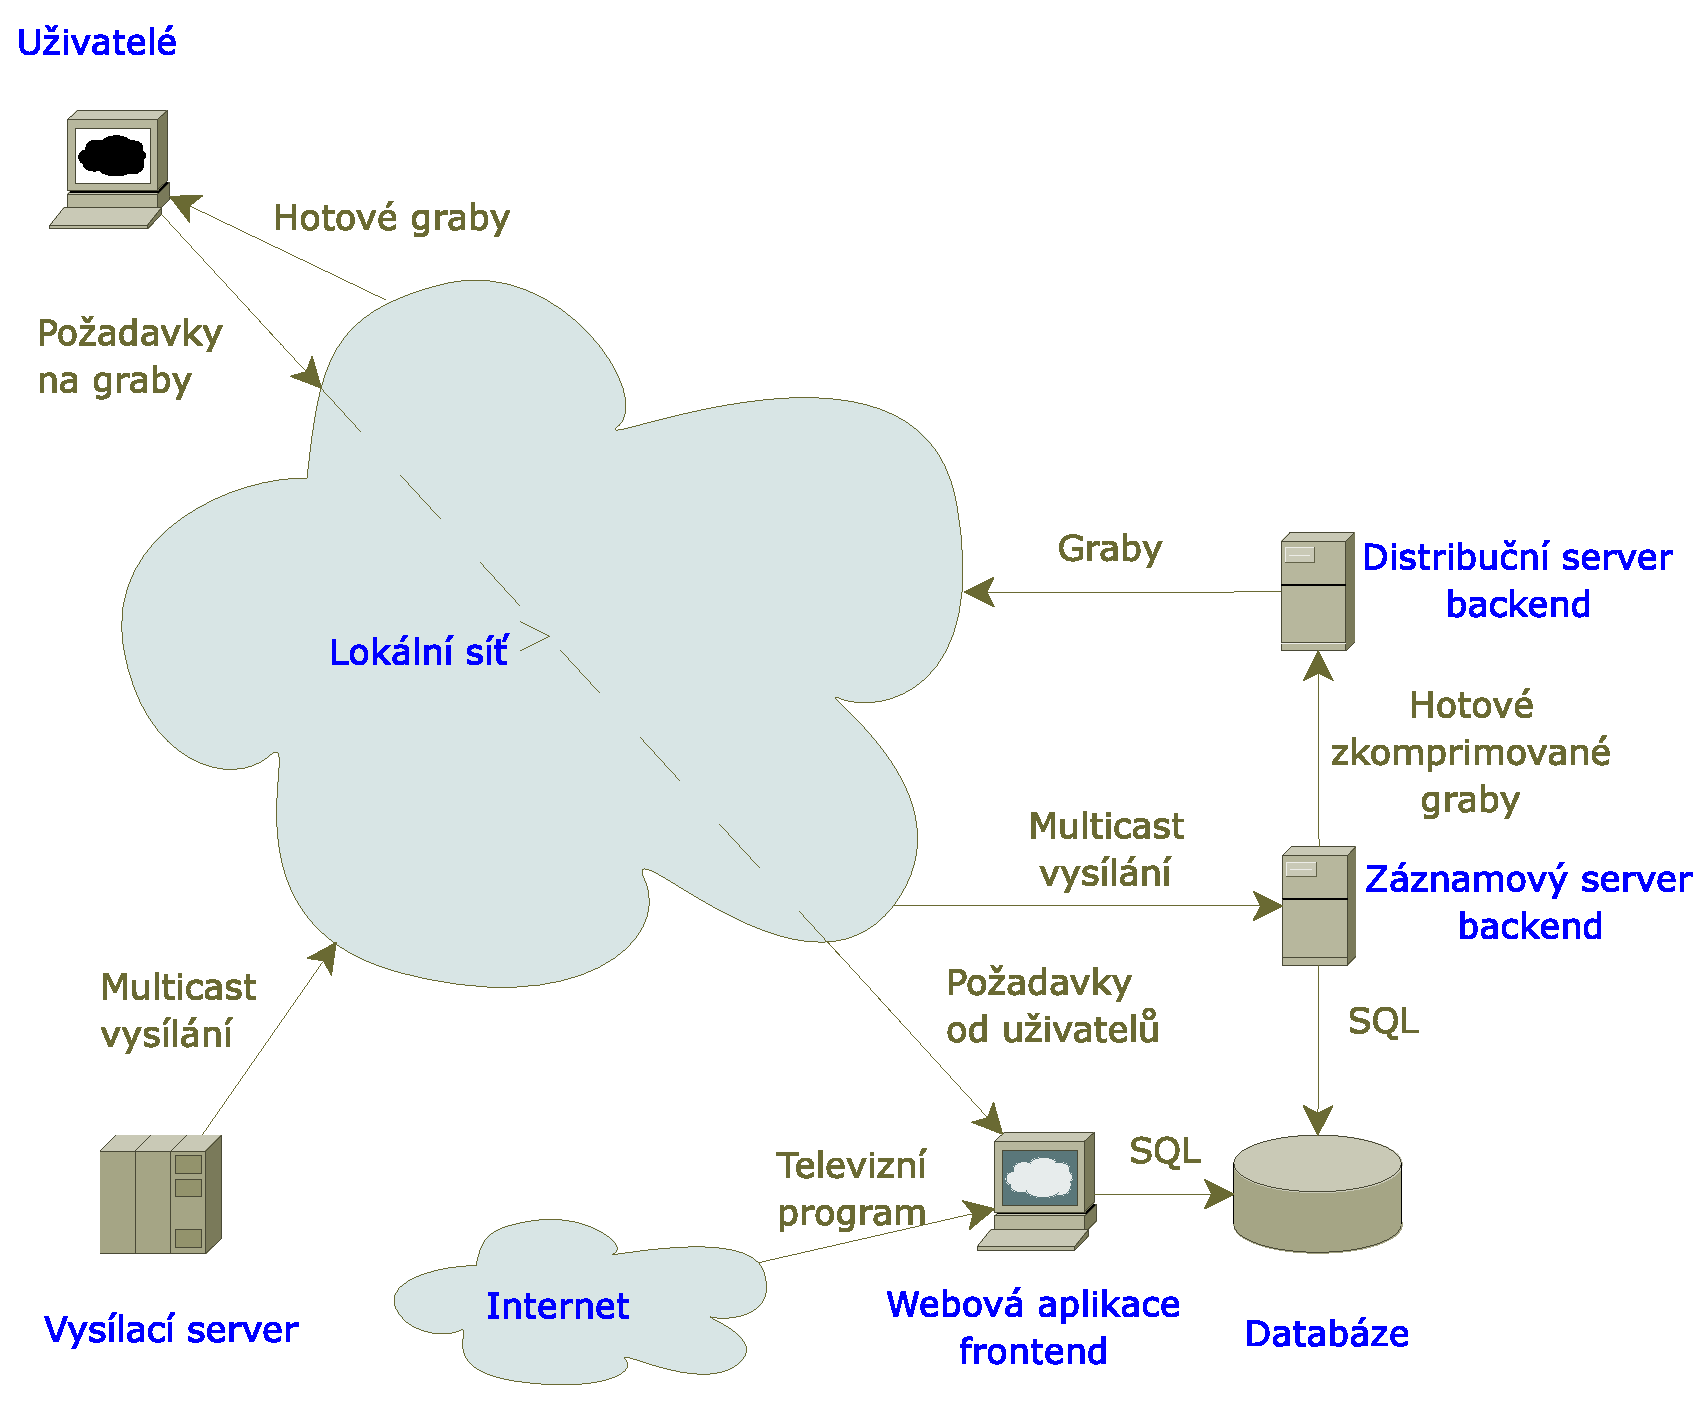
\includegraphics[width=15cm]{images/dvbgrab.eps}
\caption{Systém DVBgrabu}
\label{fig:overview}
\end{center}
\end{figure}

Pro funkci systému potřebujeme audio-video signál přenášený po lokální síti, zdroj televizního programu pro všechny nahrávané TV kanály. Uživatel poté objednává nahrávku (grab) pouhým kliknutím na název pořadu. Hotová nahrávka se komprimuje do uživatelem preferovaného formátu a výsledek je poté připraven ke stažení. O dostupnosti nové nahrávky je uživatel, který si ji objednal, informován e-mailem.
\vfill
\pagebreak
\section{Vlastnosti DVBgrabu}
\bitem
\item Podpora distribuce nahrávek také přes HTTP server apache
\item Webové konfigurační rozhraní setup.php
\item Sjednocená a centralizovaná konfigurace v jednom souboru config.php
\item Možnost volby preferovaného formátu hotové nahrávky (MPEG-2, MPEG-4, ...)
\item Možnost nahrávat z několika kanálů paralelně, odpadá potřeba volit, který z analogových kanálů bude naladěn v době záznamu
\item Záznamové skripty pracující s libovolným audio-video signálem šířeným po lokální síti
\item Využití ADOdb pro abstraktní přístup k téměř libovolnému databázovému stroji
\item Seznam hotových nahrávek ve webovém rozhraní obsahuje i odkazy na stažení
\item Objednávání nahrávek přímo z vyhledávacího formuláře
\item Možnost dodatečných změn nastavení uživatelského účtu, případně zrušení účtu
\item Zasílání nového hesla při zapomenutí starého
\item Kompletní vícejazyčná podpora
\item K dispozici kromě češtiny je také angličtina, francouzština a slovenština
\item Automatický výběr použitého jazyku ve webovém rozhraní
\item Podpora načítání TV programu ve formátu XMLTV
\item Automatická údržba záznamového serveru
\item Podpora zobrazování detailních záznamů až při požadavku pomocí asynchronních XMLHTTP požadavků
\item Detailní informace o pořadu k dispozici společně s nahrávkou ve formátu XML s připojenou XSL transformací.
\eitem

\section{Servery}
Systém využívá ke svému běhu 2 různé servery, i když to není nutností. Na jednom běží databáze a webové rozhraní. Na druhém potom vysílání signálu do lokální sítě, záznam na disk a distribuce nahraných pořadů.
\section{Databáze}
Jako databázový server lze použít téměř libovolnou SQL databázi, protože systém využívá knihovnu ADOdb, která podporuje v současné době zhruba 15 různých databázových strojů. Systém byl provozován na MySQL databázi, nyní na PostgreSQL. Kvůli použití ADOdb je nutné vždy volat SQL kód jen s použitím ADOdb funkcí, například pro formátování datumu v SQL dotazech musí být vždy volána odpovídající ADOdb funkce, která vygeneruje funkci odpovídající aktuálně použitému databázovému serveru.
\section{Webové stránky}
Webové prostředí je napsáno pomocí XHTML+PHP+JavaScript. Obsahuje jak uživatelské tak administrativní rozhraní převážně pro prvotní nastavení a případné změny v konfiguraci. Je napsáno s podporou více jazykových variant (čeština, slovenština, angličtina, francouzština). Všechny zobrazované texty jsou definovány jako konstanty v souborech lang/lang.jazyk.php.

Jazyk se volí postupně podle těchto pravidel:
\bitem
\item podle cookie, pokud uživatel někdy přepnul jazyk ručně kliknutím na ikonu vlajky
\item podle preferovaných jazyků v nastavení prohlížeče
\item v databázi hledáme poslední použitý jazyk daného uživatele
\item výchozí jazyk definovaný v globální konfiguraci 
\eitem

Nakonec se zvolený jazyk uloží do databáze k uživateli jako poslední použitý jazyk. To se využívá například při odesílání e-mailu o úspěšném nahrání, kdy nemáme již k dispozici uživatele, jeho cookies ani jeho prohlížeč.

Z důvodu vícejazyčného webového rozhraní je třeba zajistit také kódování v databázi nastavené na UTF-8, aby podporovala všechny přípustné varianty.

\section{Záznam}

O nahrávání se starají 2 nekonečné smyčky naprogramované také v PHP. Jedna se stará \linebreak[4]o~záznam (grab\_loop), druhá o komprimaci (encode\_loop). Záznamová smyčka se spouští po startu systému a v krátkych časových intervalech kontroluje, zda na některém kanálu nezačíná nějaký objednaný pořad. 
Pokud ano, spustí na pozadí nový proces, který zajistí záznam tohoto pořadu (grab\_process, kterému se předává pouze ID záznamu v databázi) a sama pokračuje dál ve své činnosti.

Komprimační smyčka je odlišná, spouští se sice také po startu systému, ale protože nemá smysl pouštět paralelně příliš mnoho komprimačních procesů, tak vždy kontroluje, zda existuje v~databázi nějaký nevyřízený požadavek na formát, do kterého se zrovna nic nekomprimuje. Pokud ano, vybere nejstarší podle data vysílání pořadu a spustí nový proces (encode\_process, kterému předává ID požadavku a formát, jaký se má použít). To znamená, že kolik různých formátů si uložíme do databázové tabulky encoder, tolik komprimačních procesů může běžet paralelně.

Vlastní záznam na disk je prováděn pomocí programu dumprtp, z balíku dvbstream, který ukládá datový tok ze zadané IP adresy a portu do souboru. V záznamovém procesu se nejdříve všechny požadavky na daný pořad přepnou ze stavu \quotedblbase naplánován'' do stavu \quotedblbase ukládá se''. Poté je dumprtp spouštěn jako volání podprocesu na pozadí a poté je počítán čas až do konce pořadu, kdy se pošle procesu dumprtp signál TERM k ukončení. 

Data se při ukládání netransformují, takže zůstanou uložena jako MPEG-TS (transport stream). To umožňuje paralelní zápis několika pořadů na disk, protože je to operace relativně nenáročná. Transport stream je optimalizovaný spíše pro přenos audio-video signálů, než pro jejich přehrávání (neobsahuje příliš často klíčové snímky, takže například při posunech je dlouhá odezva než se obnoví obraz). Z jaké IP adresy a portu se má ukládat, je nyní určeno v databázi v definici televizního kanálu.

Jmenné konvence pro název nahrávky jsou DVB- jako předpona, pak datum ve formátu Ymd-Hi (rok, měsíc, den, hodiny, minuty) tak, aby se adresář s nahrávkami dal řadit chronologicky podle abecedy. Dále následuje jméno kanálu (po odstranění diakritiky) a název pořadu, buď po odstranění diakritiky nebo jenom ID záznamu, pokud to je v konfiguraci nastaveno (přesné jméno pořadu včetně diakritiky je pak až v popisném XML souboru, viz dále. Nekomprimované nahrávky mají příponu .ts jako transport stream.

Po ukončení dumprtp smyčka ještě zkontroluje, zda má nahrávka nějakou odpovídající nenulovou velikost a informace o uložení se aktualizuje v databázi (všechny požadavky na tento pořad přejdou ze stavu \quotedblbase ukládá se'' do stavu \quotedblbase uložen''.

\section{Specifika ukládání z digitálního vysílání}
Součástí DVB vysílání jsou i informace o vysílaných pořadech.

Tyto informace jsou vysílány jako součást MPEG-2 dat pomocí protokolu PMCP (Programming Metadata Communication Protocol), což jsou do XML balené data z PSIP (Program and System Information Protocol).

Součástí PSIP jsou následující tabulky:
\bitem
\item \textbf{STT} (system time table) -- aktuální čas vysílaný každou sekundu
\item \textbf{MGT} (master guide table) -- datové ukazatale do dalších tabulek PSIP
\item \textbf{VCT} (virtual channel table) -- seznam kanálů a přiřazení jejich čísel
\item \textbf{RRT} (rating region table) -- hodnocení obsahu pro jednotlivé regiony
\item \textbf{EIT} (event information table) -- názvy a další data pro televizní program
\item \textbf{ETT} (extended text table) -- detailní popis programů
\item \textbf{DCCT} (directed channel change table)
\item \textbf{DCCST} (directed channel change selection code table)
\eitem

Tabulky EIT a ETT používá v MHP (Multimedia Home Platform -- aplikační rozšíření v DVB) aplikace EPG (Electronic program guide -- elektronický televizní program). Tyto informace by bylo velmi výhodné použít pro přesné nastavení začátku a konce záznamu.

Pokud toto nemáme k dispozici, musí nahrávání začínat několik minut před plánovaným začátkem pořadu (lze konfigurovat kolik) a také lze nastavit, kolik minut se má nahrávat po plánovaném konci pořadu.

Pokud bychom chtěli využít informace z EIT přímo v DVBgrabu, tak bychom museli nejdříve zajistit jejich distribuci z vysílajícího serveru do lokální sítě.

Podle zástupců Czech Digital Group jsou prý tyto údaje již dostupné. Pokud jim televize údaje dodá, tak je pouze převedou do formátu vhodného pro EIT a vloží do toku dat.

Pokud by v EIT byly obsaženy i značky začátku a konce televizní reklamy, tak by šlo podle nich vypínat a zapínat záznam, a tím tedy zajistit automatické vystřihování reklamy. Případně by bylo možné naprogramovat nějaký vlastní algoritmus pro poznávání reklamy (třeba podle podobnosti s dodanou počáteční a koncovou znělkou). Tento algoritmus by byl pravděpodobně dosti hardwarově náročný, což by při několika paralelních záznamech mohlo vést až ke ztrátám snímku, proto nebyl použit. Tyto algoritmy také nemusí být v souladu se zákonem (automatický systém na vystřihování reklamy byl součástí software DVD rekordérů KISS a~musel být odstraněn a~zůstalo pouze automatické přetáčení reklamy při sledování ze záznamu).
\vfill
\pagebreak
\section{Komprimace záznamů}
Komprimační smyčka postupně prochází přes všechny formáty (encodery) a zkoumá, zda pro ty, které aktuálně neběží (nemají v databázi uložené své číslo procesu PID, pokud je uloženo, tak se testuje, zda doopravdy běží), neexistuje nějaký čekající požadavek ve stavu \quotedblbase uložen''. Pokud ano, vybere opět nejstarší. Založí na pozadí nový proces, který komprimaci zajistí. Komprimační proces nejdříve opět změní stav požadavku~v databázi z \quotedblbase uložen'' na \quotedblbase komprimuje se''.
 
Poté spustí skript, jehož jméno je opět uvedeno v~databázi a který musí být uložen v adresáři encoders. Tomuto skriptu předá název nahraného pořadu, který do databáze uložil předcházející záznamový proces, a z původního jména vytvoří název cílového souboru připojením definované přípony z databáze. Po úspěšné komprimaci je z .ts souboru vytvořen například .avi soubor ve formátu MPEG-4, poté se znovu zkontroluje, zda výsledný soubor má odpovídající velikost, a~pokud ano, dojde k uveřejnění nahrávky požadujícím uživatelům. 

\section{Komprimační formáty}
Komprimaci zajišťuje program mencoder, který podporuje velmi mnoho formátů. Některé základní jsem uvedl v příloze.
Čím více kombinací kontejner, video, audio kodeků umožníme uživateli zvolit, tím větší budou nároky na čas a místo na disku. Každá nahrávka totiž musí být zkomprimována do všech uživateli požadovaných variant a také bude ve všech požadovaných variantách uložena na vyhrazeném diskovém prostoru.

Proto je připraveno pouze pár zajímavých kombinací, a to:

\bitem
\item \textbf{MPEG-2 TS} -- formát v jakém přijímáme DVB signál ze sítě, soubor bude mít příponu .mpg.
\item \textbf{AVI/MPEG-4 ASP (z libavcodec)/MP3} -- běžně používaný komprimovaný soubor, hodina záznamu odpovídá zhruba 700MB. Jsou předdefinované varianty s různým měřítkem (různé rozlišení), soubor bude mít příponu .avi.
\eitem
Dále by bylo vhodné použít:
\bitem
\item \textbf{OGG/Theora/Vorbis} -- svobodná obdoba předchozí kombinace s mírně efektivnějším poměrem kvality a velikosti souboru, s příponou .ogg.
\item \textbf{MP4/MPEG-4 AVC (z x264)/AAC} -- nejvyšší kvalita, pokud budeme mít dostatečně kvalitní zdroj, přípona by byla .mp4. Tato varianta bude trvat mnohem déle, proto je vhodná jen pro výkonnější servery nebo tam, kde nevadí časový rozdíl mezi koncem pořadu a uveřejněním grabu.
\eitem
\section{Uveřejnění nahrávky}
\subsection{Popisný XML soubor}
Je vytvářen XML soubor popisující detaily nahrávky. Obsahuje název pořadu s diakritikou, název kanálu s diakritikou, začátek a konec pořadu podle televizního programu, začátek a konec nahrávání, použitý komprimační formát, výslednou velikost souboru v kB a MD5 součet pro kontrolu bezchybného stažení.

XML soubor je ve webovém prohlížeči zobrazován v podobě přehledné tabulky, která je z XML souboru vytvořena podle XSL šablony.

Ta je v uživatelském adresáři vygenerována (podle jazyku, který uživatel používá na webovém rozhraní DVBgrabu) v souboru dvbgrab.xsl. Pokud uživatel chce stejně zobrazovat i stažené XML soubory, musí k nim do adresáře zkopírovat i tento soubor.

\subsection{Vytvoření symbolického odkazu}
Vytvoření symbolického odkazu z uživatelova adresáře do sdíleného prostoru, ve kterém jsou uložené všechny nahrávky (jak na nahrávku, tak na odpovídající XML soubor).

\subsection{Kontrola a případné založení uživatelského adresáře}
Během vytváření symbolických odkazů dojde také ke kontrole, zda je uživatelský adresář již založen a případně také k přegenerování souboru .htaccess, který určuje ze kterých IP adres smí uživatel své nahrávky stahovat (tato IP adresa je vždy pouze jedna a je uložena v databázi u~informací o uživateli). Uživatel má možnost přes webové rozhraní zadat její změnu, proto musí docházet k přegenerování těchto .htaccess souborů. Druhá varianta je přegenerování souboru pouze pokud nějaká změna skutečně nastala, což rozhoduje údržbový skript pouštěný pomocí plánovače cron. 

Oba přístupy mají své výhody, ale i nevýhody. První je nevýhodný například pro uživatele, který při pokusu o stažení nahrávky zjistí, že má zaregistrovanou neaktuální IP a další nahrávku zatím neplánuje. Druhý naopak nepotěší uživatele, který ráno zadá změnu IP, v poledne se mu uloží nahrávka a až do půlnoci nejde stáhnout, když se údržbové skripty budou pouštět jen 1x denně o půlnoci. Řešením je buď dostatečně časté pouštění údržby nebo kombinace obou přístupů. Výchozí nastavení generuje .htaccess soubory v obou případech.

\subsection{Odeslání e-mailu a označení v databázi}
Odeslání informačního e-mailu všem uživatelům, kteří tuto nahrávku v tomto formátu požadovali. U všech uživatelských požadavků je v databázi nastaveno jméno souboru s nahrávkou, jak bude přístupná přes http server, což je pak použito pro generování odkazů na stažení v sekci \quotedblbase moje graby''.

\section{Distribuce záznamů}
Distribuce nahrávek mezi uživatele je zajištěna přes http server apache (nyní ve verzi 2.2.x, která již nemá problémy se soubory většími než 2GB). Alternativně lze použít i nějaký ftp server, který umí autentifikovat uživatele nejlépe proti použité databázi. Pokud potřebujeme generovat uživatelské účty pro ftp server, máme k dispozici pouze uživatelská jména a md5 součty jejich hesel (musíme číst i md5 hesel z externí autorizační databáze).

\section{Získávání aktuálního televizního programu pro web}
Stahování aktuálního TV programu je zajištěno přes různé moduly. V adresáři tvgrabbers jsou jednotlivé php skripty. V distribuci je skript tv\_grab\_novinky\_cz/tv\_grab\_novinky\_cz.php, který načítá data ze serveru novinky.cz. Stažený html kód je zpracován pomocí regulárních výrazů a jednotlivé pořady jsou uloženy do databáze. Tento skript umí pouze několik programů (ČT1, ČT2, Nova, Prima), pro načítání jiných je nutné skript editovat.

XMLTV -- dalším skriptem v distribuci je xmltv\_to\_db.php, který lze použít pro vkládání XML souboru ve formátu XMLTV do databázové tabulky television. Nejdříve se podíváme, co je to XMLTV. XMLTV je specifikace, jak zapisovat televizní program do XML souborů. Tuto specifikaci využívá velmi mnoho programů viz. \cite{xmltvURL}. Na stránkách XMLTV lze stáhnout též instalační balík, který obsahuje stahovací skripty pro poměrně mnoho zemí. Bohužel není obsažen skript po Českou republiku z důvodu, který uvedu v následující sekci.

Každý stahovací skript musí být před prvním použitím spuštěn v konfiguračním řežimu (např. pro skript tv\_grab\_cz takto \quotedblbase tv\_grab\_cz -conf''). Konfigurace se obvykle skládá z několika obecných dotazů. Dále se vypisuje seznam televizních kanálů, které umí stahovat, a pro každý kanál uživatel volí, zda se má stahovat, či ne. Poté stačí spustit skript s parametrem udávajícím na kolik dnů dopředu má stahovat, případně od kolikáteho dne začít (\quotedblbase tv\_grab\_cz --days 10'', stáhne na 10 dní dopředu pro všechny povolené kanály jejich program). Výstupem skriptu je správně formátovaný soubor XML, který ještě potřebujeme transformovat do databáze.

Protože se nám hodí i koncové časy pořadů, pomůže nám pomocný skript z balíku XMLTV tv\_sort, který nejen chronologicky seřadí pořady v rámci kanálu, ale také každý pořad doplní koncovým časem (podle počátečního času chronologicky následujícího pořadu). Bohužel tohle selhává u posledních pořadů v rámci dne, kdy následujícím pořadem je až první ranní pořad dalšího dne. Tyto situace se snaží detekovat systém až při vytváření požadavku na nahrání a~pokud pořad začíná mezi 1. a 5. hodinou ranní a trvá déle než 4 hodiny, tak se koncový čas nastaví jen na čas počáteční + definovaná konstanta (výchozí hodnota je +2 hodiny). Pokud koncové časy nemáme v databázi vůbec (např. po použití modulu tv\_grab\_novinky\_cz.php), tak se koncový čas určuje také při vytváření požadavku na nahrání.

Takto předzpracovaný program již můžeme zpracovávat pomocí skriptu xmltv\_to\_db.php. Ten složí pro každý element <programme> 2 SELECT dotazy, INSERT pro vložení a UPDATE pro aktualizaci. První dotaz zjistí, zda v danou dobu na daném kanálu již existuje v databázi pořad se stejným jménem, a pokud ano, element je ignorován. Jinak se provede druhý dotaz, který zjišťuje, zda neexistuje v tu dobu pořad s jiným jménem. Pokud ano, použije se vygenerovaný UPDATE, pokud ne, použije se INSERT. Pokud se ve vstupním souboru objeví například pořad na kanálu, jehož xmltv id nemáme v databázi DVBgrabu registrováno, vypíše se varování a pořad se také nevkládá.

\section{Právní aspekty získávání televizního programu z veřejně dostupných webových stránek}
V zahraničí je běžné, že dostupnost XMLTV formátu programu je částečně podporovaná i~státem. 

U nás tomu bohužel tak není a kvůli tomu v XMLTV distribuci stahovací skript pro Českou republiku v dohledné době asi nenajdeme. Dokonce tam jistou dobu byl již i obsažen. Bohužel firma provozující servery, které sloužily jako zdroj programu pro jinou firmu, která zajišťovala transformaci z HTML formátu do XMLTV, nebyla této aktivitě příznivě nakloněna, a tak byl projekt českého XMLTV pod hrozbou žaloby zastaven.

Bohužel i mně jako tvůrci DVBgrabu byla zaslána žádost o urychlené odstranění načítání televizního programu ze stránek http://www.ceskenoviny.cz, jejichž provozovatelem je Česká tisková kancelář (ČTK), jinak by záležitost řešilo právní oddělení ČTK. Proto nová verze DVBgrabu bude distribuována bez českého XMLTV modulu. Správce systému je pak nucen použít skript tv\_grab\_novinky\_cz.php (za předpokladu, že snad přátelštější provozovatel http://www.seznam.cz nepřijde s žádostí o odstranění) a nebo si zajistit xmltv zdroj svépomocí.

Doufejme, že si některý portál nabízející online TV program v HTML podobě co nejdříve všimne na trhu tohoto nedostatku a doplní své portfolio služeb například o placený přístup k XMLTV formátu svého programu.
\vfill

\chapter{Vysílání do počítačové sítě}
Pro DVBgrab potřebujeme nějaký dostatečně stabilní zdroj televizního vysílání po lokální síti. To může běžet na druhém serveru, ale může být i úplně nezávislé na DVBgrabu.

\section{Digitální vysílání v České republice}
V současné době v České republice vysílají DVB signál organizace Czech Digital Group a.s. (CDG), RADIOKOMUNIKACE a.s. (dříve ČESKÉ RADIOKOMUNIKACE a.s., zkraceně CRA) a Český Telecom a.s. (CTc). Každá organizace představuje jeden multiplex, což v DVB znamená balík televizních, rozhlasových a datových kanálů, který je vysílán v rámci jedné frekvence po~celém území.

Multiplex CRA je nyní zaměřen na pořady České televize (ČT1, ČT2, ČT24, ČT4 Sport), dále obsahuje TV Nova a 7 radiových programu Českého rozhlasu, CDG obsahuje televizi Prima, Top TV, TA3, Óčko, 24cz, TV NOE a radio Proglas, Evropa 2 a Classic. CTc měl Českou Televizi, Očko, Novu, nyní již jako Telefonica O2 vysílá pouze testovací datové toky DVB-T ve formátu MPEG-4 a testují vysílání s vysokým rozlišením HDTV.

\section{Varianty digitálního vysílání}
\begin{table}[ht]
\begin{center}
\begin{tabular}{|c|l|l|l|}
\hline
\bf{Varianta} & \bf{Použití} & \bf{Video kodek} & \bf{Modulace} \\
\hline
$DVB-T$ & pozemní & MPEG-2 & QFDM,QPSK,QAM+\\
\hline
$DVB-S$ & satelitní & MPEG-2 & QPSK+\\
\hline
$DVB-C$ & kabelové & MPEG-2 & QAM+\\
\hline
$DVB-H$ & přenosné zařízení & MPEG-4 AVC & QFDM,QPSK,QAM+\\
\hline
\end{tabular}
\end{center}
\caption{Varianty DVB vysílání}
\label{tab:tab1}
\end{table}

Variantu volíme podle dostupnosti v naší lokalitě, v Praze je nejsnazší využít variantu DVB-T (pozemní).

Pokrytí Prahy signálem DVB-T je velmi dobré, přesto se mohou objevit problémy s použitými zesilovači, které jsou obvykle vyladěny pro zesilování frekvencí běžných pro analogové televizní vysílání a frekvence DVB-T (nad 500MHz) účinně ořezávají. Proto je v případě špatného příjmu jako první potřeba zkontrolovat použité zesilovače.

Systém, který běží na Masarykově koleji ČVUT, používá signál ze 2 DVB-T karet, jedna je naladěna na multiplex CDG a druhá na CRA. 

Grabovací systém bude samozřejmě fungovat na libovolné kombinaci digitálních, ale i jinak získaných signálů, které se dají vysílat po lokální síti.

\section{Programy na vysílání}
Pro vysílání po síti se používají programy z projektu VideoLAN \cite{videolanURL}. Jejich použití je následující:

\begin{figure}[ht]
\begin{center}
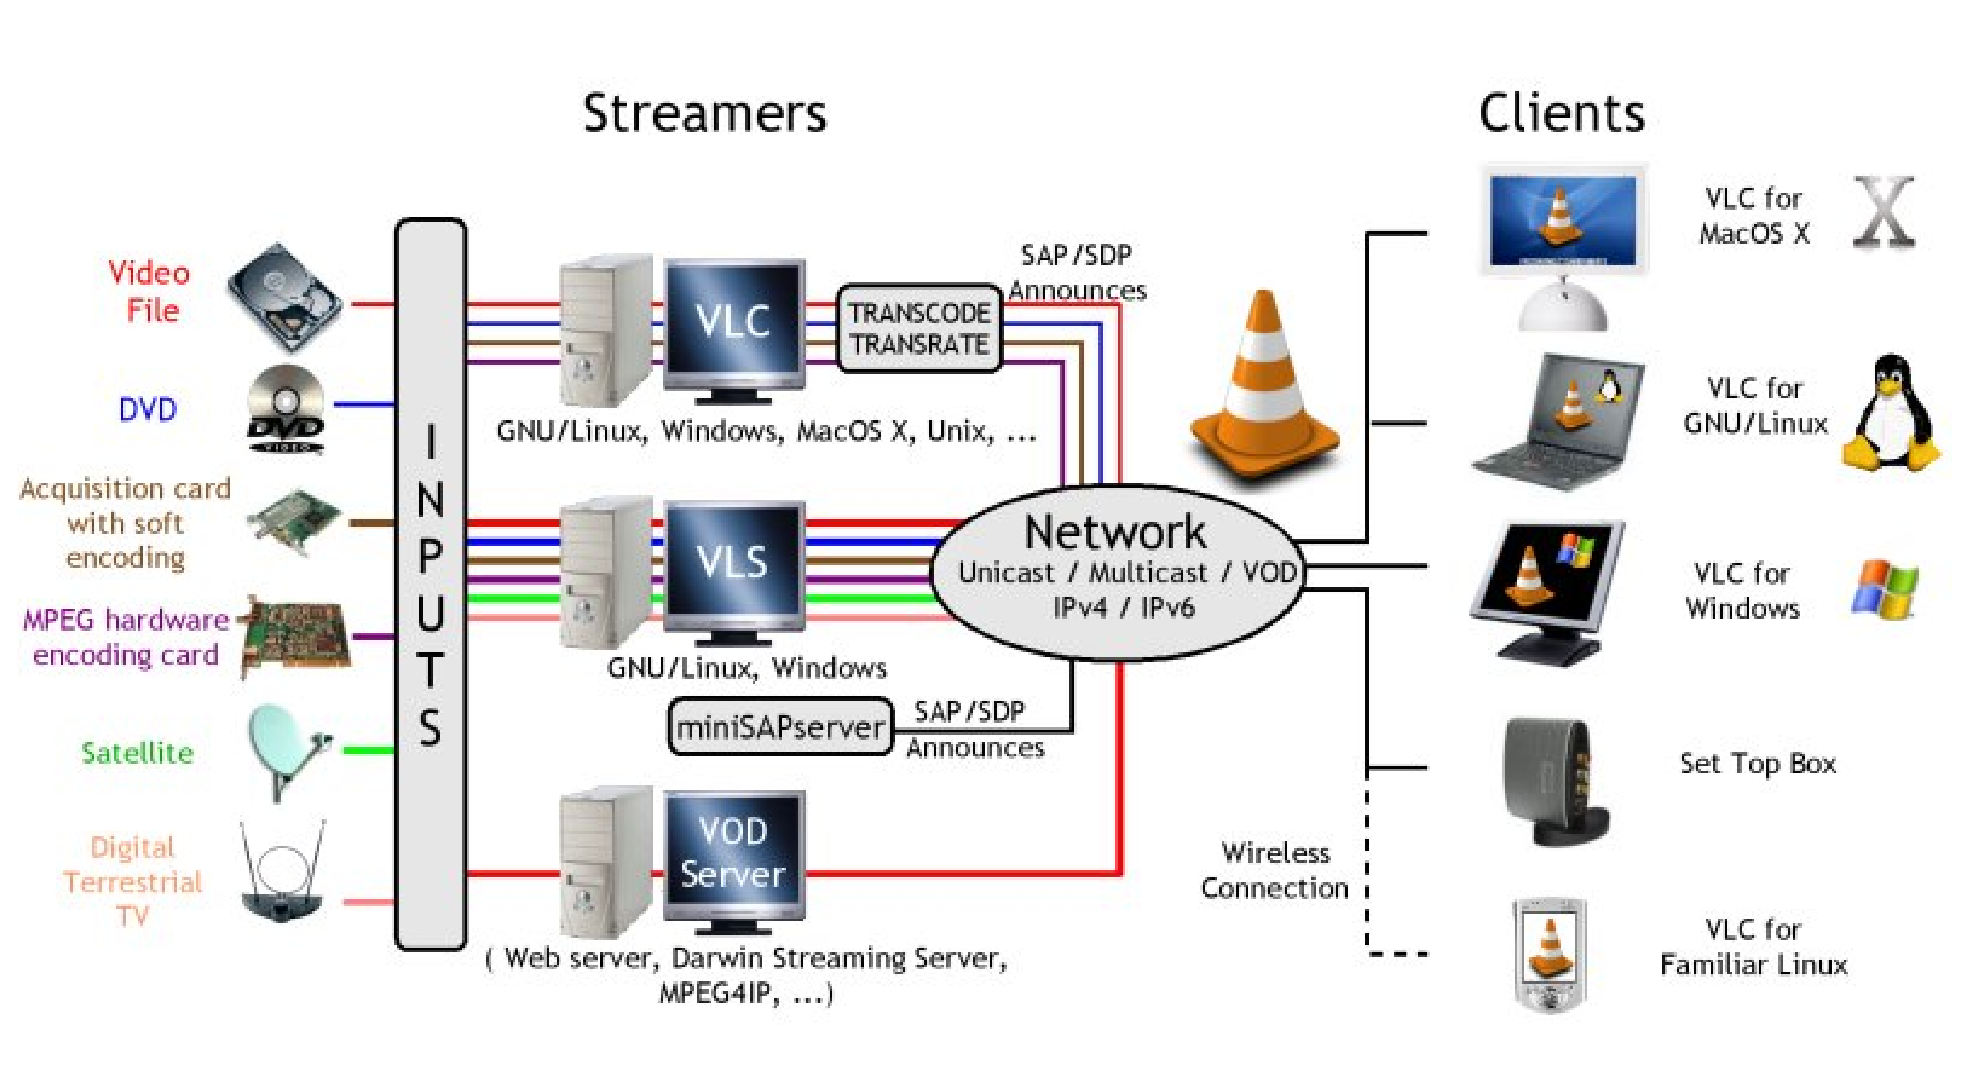
\includegraphics[width=15cm]{images/videolan}
\caption{Využití programů z projektu VideoLAN}
\label{fig:videolan}
\end{center}
\end{figure}

\section{Potřebný hardware a ovladače}
Budeme potřebovat nějaké DVB-T karty, obvykle do slotu PCI.

Odzkoušené a ověřené jsou například karty Hauppauge WinTV-NOVA-T (Technotrend Systemtechnik GmbH Technotrend-Budget, Philips Semiconductors SAA7146 rev 01).

Pokud chceme paralelně vysílat kanály z více různých multiplexů, potřebujeme více těchto karet.

Každá DVB-T karta má potom na svém tuneru naladěnu frekvenci multiplexu a paralelně přijímá všechny kanály tohoto multiplexu.

Ovladače těchto karet jsou k dispozici na stránkách projektu linuxtv \cite{linuxtvURL} a také jsou součástí jádra systému řady 2.6. V novějších jádrech než 2.6.9 se promítlo mnoho změn v ovladačích, proto je potřeba stáhnout i novější verzi firmware karty, která se nahrává při načítání ovladače.

Pro zprovoznění vysílání je vhodné nainstalovat ještě několik uživatelských aplikací jako media-tv/linuxtv-dvb, linuxtv-dvb-apps, linuxtv-dvb-headers, libdvbpsi, dvbsnoop pro Gentoo nebo dvb-utils, dvbsnoop, dvbstream, dvbtune, libdvb-dev, libdvbpsi3, libdvbpsi3-dev pro Debian.

\section{Získání seznamu dostupných kanálů}

Získání seznamu pořadů v multiplexu popíšu již v této sekci, i když daný postup lze zjednodušit, pokud použijeme přímo VideoLanClient(VLC) místo složitější kombinace VideoLanServer(VLS)+miniSAPserver.

Pro zjištění dostupných kanálů lze použít například příkaz scan z balíku dvb-utils. Nejdříve je třeba připravit soubor s výchozím nastavením tuneru, aby karta věděla, ve kterém multiplexu chceme kanály vyhledávat.

Výchozí nastavení pro různé multiplexy lze obvykle získat z www stránek provozovatele. Současný stav viz tabulka \ref{tab:mplexy}.

\begin{table}
\begin{center}
\begin{tabular}{|c|l|l|l|}
\hline
\bf{Parametr} 		& \bf{Multiplex A} 	& \bf{Multiplex B} 	& \bf{Multiplex C} 	\\
			& 	\bf{CRA} 	& 	\bf{CDG} 	& 	\bf{CTC} 	\\
\hline
Typ multiplexu		&	T		&       T		&       T		\\
\hline
Frekvence v Praze	&	506 000 000	&       674 000 000	&       818 000 000	\\
\hline
Šířka pásma		&	8 MHz		&       8 MHz		&       8 MHz		\\
\hline
Vysílací mód		&	8K		&       8K		&       8K		\\
\hline
Ochranný interval 	&	1/8		&       1/16		&       1/8		\\
\hline
Kódový poměr(fec\_hi)	&	2/3		&       2/3		&       2/3		\\
\hline
Kódový poměr(fec\_lo)	&	2/3		&       1/2		&       2/3		\\
\hline
Modulace		&	64 QAM		&       64 QAM		&       64 QAM		\\
\hline
Celková bitová rychlost	&	22,12 Mbit/s	&	23,42 Mbit/s	&	22,170 Mbit/s	\\
\hline
Kódování češtiny pro EPG&	ISO 6937	&	ISO 6937	&	ISO 8859-2	\\
\hline
Hierarchický mód 	&	ne		&       ne		&       ne		\\
\hline
\end{tabular}
\end{center}
\caption{Parametry vysílání pro jednotlivé multiplexy}
\label{tab:mplexy}
\end{table}

Takže výchozí nastavení pak vypadá následovně (můžeme zadat všechny multiplexy najednou do jednoho souboru a někdy je takový soubor již součástí instalačního balíčku s programem pro skenování):

\begin{small}
\begin{verbatim}
# DVB-T Praha (Prague, Czech Republic)
# T freq bw fec_hi fec_lo mod transmission-mode guard-interval hierarchy
T 506000000 8MHz 2/3 2/3 QAM64 8k 1/8 NONE
T 674000000 8MHz 2/3 1/2 QAM64 8k 1/16 NONE
T 818000000 8MHz 2/3 1/2 QAM64 8k 1/8 NONE
\end{verbatim}
\end{small}

Výstup programu scan poté pro České radiokomunikace (CRA) vypadá např. takto:
 
\begin{small}
\begin{verbatim}
CT1:506000000:INVERSION_AUTO:BANDWIDTH_8_MHZ:FEC_2_3:FEC_2_3:QAM_64: \
  TRANSMISSION_MODE_8K:GUARD_INTERVAL_1_8:HIERARCHY_NONE:513:641:1
CT2:506000000:INVERSION_AUTO:BANDWIDTH_8_MHZ:FEC_2_3:FEC_2_3:QAM_64: \
  TRANSMISSION_MODE_8K:GUARD_INTERVAL_1_8:HIERARCHY_NONE:514:642:2
CT24:506000000:INVERSION_AUTO:BANDWIDTH_8_MHZ:FEC_2_3:FEC_2_3:QAM_64: \
  TRANSMISSION_MODE_8K:GUARD_INTERVAL_1_8:HIERARCHY_NONE:515:643:3
Nova:506000000:INVERSION_AUTO:BANDWIDTH_8_MHZ:FEC_2_3:FEC_2_3:QAM_64: \
  TRANSMISSION_MODE_8K:GUARD_INTERVAL_1_8:HIERARCHY_NONE:516:644:4
Praha:506000000:INVERSION_AUTO:BANDWIDTH_8_MHZ:FEC_2_3:FEC_2_3:QAM_64: \
  TRANSMISSION_MODE_8K:GUARD_INTERVAL_1_8:HIERARCHY_NONE:0:658:18
Vltava:506000000:INVERSION_AUTO:BANDWIDTH_8_MHZ:FEC_2_3:FEC_2_3:QAM_64: \
  TRANSMISSION_MODE_8K:GUARD_INTERVAL_1_8:HIERARCHY_NONE:0:659:19
D-dur:506000000:INVERSION_AUTO:BANDWIDTH_8_MHZ:FEC_2_3:FEC_2_3:QAM_64: \
  TRANSMISSION_MODE_8K:GUARD_INTERVAL_1_8:HIERARCHY_NONE:0:661:21
Leonardo:506000000:INVERSION_AUTO:BANDWIDTH_8_MHZ:FEC_2_3:FEC_2_3:QAM_64: \
  TRANSMISSION_MODE_8K:GUARD_INTERVAL_1_8:HIERARCHY_NONE:0:662:22
Radio Cesko:506000000:INVERSION_AUTO:BANDWIDTH_8_MHZ:FEC_2_3:FEC_2_3:QAM_64: \
  TRANSMISSION_MODE_8K:GUARD_INTERVAL_1_8:HIERARCHY_NONE:0:663:23
\end{verbatim}
\end{small}

a pro Czech Digital Group (CDG) např. takto:

\begin{small}
\begin{verbatim}
CT 1:674000000:INVERSION_AUTO:BANDWIDTH_8_MHZ:FEC_2_3:FEC_1_2:QAM_64: \
  TRANSMISSION_MODE_8K:GUARD_INTERVAL_1_16:HIERARCHY_NONE:2501:2502:5
CT 2:674000000:INVERSION_AUTO:BANDWIDTH_8_MHZ:FEC_2_3:FEC_1_2:QAM_64: \
  TRANSMISSION_MODE_8K:GUARD_INTERVAL_1_16:HIERARCHY_NONE:164:96:4
NOVA:674000000:INVERSION_AUTO:BANDWIDTH_8_MHZ:FEC_2_3:FEC_1_2:QAM_64: \
  TRANSMISSION_MODE_8K:GUARD_INTERVAL_1_16:HIERARCHY_NONE:205:206:3
TOP TV:674000000:INVERSION_AUTO:BANDWIDTH_8_MHZ:FEC_2_3:FEC_1_2:QAM_64: \
  TRANSMISSION_MODE_8K:GUARD_INTERVAL_1_16:HIERARCHY_NONE:2601:2602:2
CT24:674000000:INVERSION_AUTO:BANDWIDTH_8_MHZ:FEC_2_3:FEC_1_2:QAM_64: \
  TRANSMISSION_MODE_8K:GUARD_INTERVAL_1_16:HIERARCHY_NONE:1026:1027:7
CRo 2:674000000:INVERSION_AUTO:BANDWIDTH_8_MHZ:FEC_2_3:FEC_1_2:QAM_64: \
  TRANSMISSION_MODE_8K:GUARD_INTERVAL_1_16:HIERARCHY_NONE:0:2832:6
CRo 1:674000000:INVERSION_AUTO:BANDWIDTH_8_MHZ:FEC_2_3:FEC_1_2:QAM_64: \
  TRANSMISSION_MODE_8K:GUARD_INTERVAL_1_16:HIERARCHY_NONE:0:2831:9
Proglas:674000000:INVERSION_AUTO:BANDWIDTH_8_MHZ:FEC_2_3:FEC_1_2:QAM_64: \
  TRANSMISSION_MODE_8K:GUARD_INTERVAL_1_16:HIERARCHY_NONE:0:180:11
Evropa 2:674000000:INVERSION_AUTO:BANDWIDTH_8_MHZ:FEC_2_3:FEC_1_2:QAM_64: \
  TRANSMISSION_MODE_8K:GUARD_INTERVAL_1_16:HIERARCHY_NONE:0:110:19
EXPRESRADIO:674000000:INVERSION_AUTO:BANDWIDTH_8_MHZ:FEC_2_3:FEC_1_2:QAM_64: \
  TRANSMISSION_MODE_8K:GUARD_INTERVAL_1_16:HIERARCHY_NONE:0:120:22
CLASSIC FM:674000000:INVERSION_AUTO:BANDWIDTH_8_MHZ:FEC_2_3:FEC_1_2:QAM_64: \
  TRANSMISSION_MODE_8K:GUARD_INTERVAL_1_16:HIERARCHY_NONE:0:130:23
Prima:674000000:INVERSION_AUTO:BANDWIDTH_8_MHZ:FEC_2_3:FEC_1_2:QAM_64: \
  TRANSMISSION_MODE_8K:GUARD_INTERVAL_1_16:HIERARCHY_NONE:161:84:1
\end{verbatim}
\end{small}

MPEG-2 transport stream je balíkem elementárních kanálů (MPEG-2 ES -- Elementary stream) a informačních tabulek.

Každá složka je jednoznačně určena identifikačním číslem PID (13 bitové identifikační číslo složky, unikátní v rámci multiplexu). Podle PID se určuje, které pakety patří k sobě.
\bitem
\item \textbf{PAT -- Program Association Table} je první informační tabulkou, která je vždy vysílána s~PID 0x0. Obsahuje pro každý kanál v multiplexu PID, kde je vysílána jeho PMT tabulka.
\item \textbf{PMT -- Program Map Table} je potom seznam PID jednotlivých složek. Každý kanál má vysílánu vlastní PMT tabulku na vlastním PID.
\item \textbf{PCR -- Program Clock Reference} zdroj časového signálu pro dekodér.
\item \textbf{PIDu 0x1FFF} vyhrazený pro vysílání prázdných paketů, které slouží jenom na doplnění vysílání do určité velikosti, aby byla dodržena konstantní velikost (constant bitrate).
\eitem

Příkaz scan nám tedy vypsal informační tabulky PAT a PMT. Každý řádek je tedy jednou tabulkou PMT. V prvním sloupci je název kanálu, následují parametry společné pro celý multiplex a zajímavé jsou pak poslední číselné sloupce oddělené dvojtečkou.

Úplně poslední určuje PID této PMT tabulky, což lze použít jako identifikátor kanálu.
Předcházející čísla jsou PID jednotlivých složek programu, a to v pořadí video, audio.

Přehledně je to zobrazeno na následujícím obrázku \ref{fig:PATaPMT}, převzatém z \cite{digitvURL}.
\vfill
\pagebreak

\begin{figure}[ht]
\begin{center}
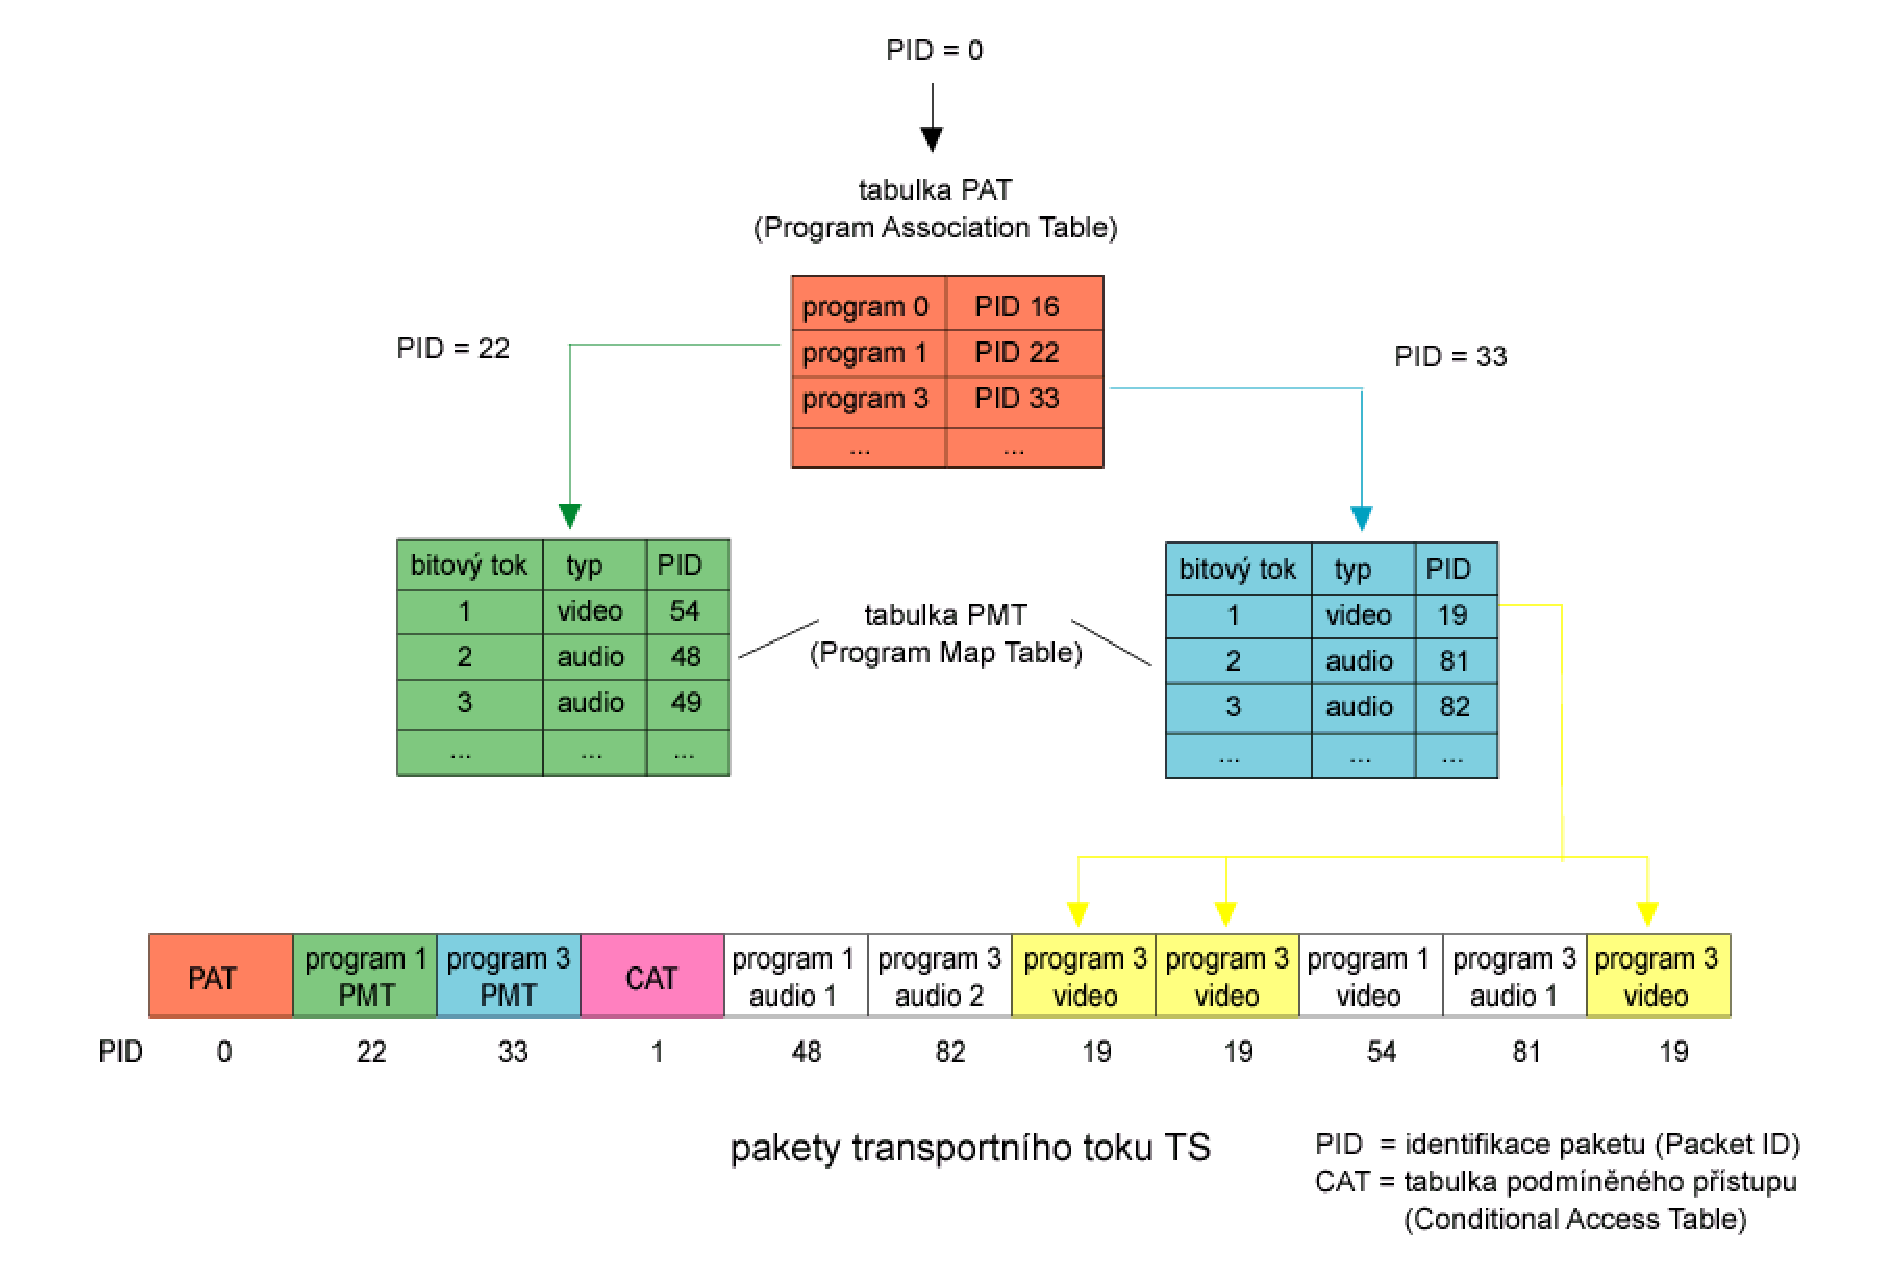
\includegraphics[width=15cm]{images/PATaPMT}
\caption{Tabulky toků v MPEG-2}
\label{fig:PATaPMT}
\end{center}
\end{figure}

\section{Metody vysílání}
Nyní tedy umíme zjistit dostupné kanály a jejich konfiguraci. Před volbou vysílacího serveru se ještě musíme rozhodnout pro metodu vysílání.
Pro provozování DVBgrabu je nejdůležitější vysílání pomocí multicastu. Multicast je totiž nejefektivnější a díky tomu vlastně jediný použitelný pro větší lokální sítě. 

\subsection{Unicast}
\bitem
\item \textbf{Popis} -- vysílání pro konkrétní IP adresu
\item \textbf{Výhody} -- snadná konfigurace pro málo uživatelů, možnost definovat povolené adresy
\item \textbf{Nevýhody} -- data se posílají tolikrát, kolik je uživatelů, což značně zatěžuje síť.
\eitem

\subsection{Multicast}
\bitem
\item \textbf{Popis} -- vysílání pro skupinu IP adres
\item \textbf{Výhody} -- do skupiny se klient může přihlašovat a odhlašovat pomocí IGMP (Internet Group Management Protocol) paketů, takže dostává data jen z těch stanic, které sleduje
\item \textbf{Nevýhody} -- pro funkční a efektivní multicast vysílání je potřeba, aby switche podporovaly IGMP snooping, což je mechanismus přeposílání packetů pouze na ty porty, ze~kterých přišel přihlašovací paket do dané skupiny. Jinak se data šíří v rámci switche jako broadcast.
\eitem
\vfill
\pagebreak
\subsection{Broadcast}
\bitem   
\item \textbf{Popis} -- vysílání na úplně všechny IP v síti
\item \textbf{Výhody} -- snadné
\item \textbf{Nevýhody} -- značné zatížení sítě, data dostávají všichni a ze všech stanic.
\eitem

\section{Seznam kanálů pro uživatele}
Když máme seznam pořadů a přidělíme jim adresy, na kterých je budeme vysílat, je vhodné vytvořit také statický playlist. Ten se bude hodit uživatelům, kteří nebudou používat přehrávač s podporou SAP playlistu. Playlist M3U je obyčejný textový soubor obvykle s příponou .m3u obsahující pro každý pořad jeho název (za EXTINF) a adresu (následující řádek), viz ukázka:

\begin{small}
\begin{verbatim}
#EXTM3U
#EXTINF:0,CRA_CT1
rtp://@239.194.12.1
...
#EXTINF:0,CRA6_CT1
rtp://@[ff08::701]
...
\end{verbatim}
\end{small}

\section{VideoLAN Server nebo VideoLAN Client?}
Pro vysílání můžeme použít buď VLS (VideoLan Server) nebo VLC (VideoLan Client). Zásadní rozdíl je ve složitosti konfigurace a udržovanosti projektu. VLS není již několik let aktivně vyvíjen, VLC už podporuje všechny jeho funkce a nyní i mnohem více.

VLS má složitějsí konfiguraci, kde je potřeba definovat správně seznam kanálů pro jednotlivé karty v souborech .dvbrc.N. Také neobsahuje integrovaný SAP server jako VLC. To pro nás znamená další práci s konfigurací SAP serveru. Vlastní konfigurace v souboru vls.cfg je sice přehledná, ale přesto dost náchylná k chybám při úpravách. Velkou výhodou VLS je jeho použití na serverech bez grafického prostředí, protože ani jeho binární balíčky nezávisí na žádných grafických knihovnách.

VLC má mnohem snažší konfiguraci a nepotřebuje .dvbrc.N soubory, což sice znamená, že nemůžeme definovat pro programy symbolické názvy, ale taky to ušetří práci s vytvářením těchto souborů, pokud se skladba programů v multiplexu častěji mění. VLC má integrovaný SAP server, takže je vše schováno přehledně v jednom souboru. Nevýhoda u binárních instalačních balíčků se dá obejít buď překompilováním VLC do balíčku bez podpory X serveru nebo například u~distribuce Gentoo záleží pouze na správné volbě USE flagů při instalaci.

\section{Popis VideoLAN Server}
Open source projekt, který umí vysílat do sítě mnoha různými způsoby a z mnoha různých zdrojů.

\subsection{Zdroje}
\bitem
\item statické soubory na disku nebo nějakém médiu (ve formátu MPEG-1, MPEG-2, MPEG-4)
\item disky DVD v DVD mechanikách
\item digitální satelitní vysílání z DVB-S karet
\item digitální pozemní vysílání z DVB-T karet
\item přímé přenosy z kamery nebo komprimační karty.
\eitem

\subsection{Výstupy}
\bitem
\item na konkrétní IP adresu -- unicast
\item na všechny adresy v určité síti -- broadcast
\item na všechny počítače, které se přihlásí k odběru dané skupiny -- multicast
\item a to vše jak ve variantě IPv4, tak v modernější IPv6.
\eitem

Hardwarové nároky jsou přibližně Pentium 100 MHz a 32MB RAM pro vysílání jednoho televizního kanálu. Pokud jsou vysílány data ze souborů na lokálním disku, tak je větším omezením čtecí rychlost disku a síťové připojení.

VLS lze používat jak ve verzi pro MS Windows, tak pro Linux. K dispozici jsou samozřejmě i~zdrojové kódy.

Instalační binární i zdrojové balíčky jsou ke stažení na adrese \cite{videolanURL}.
Linuxové distribuce obvykle obsahují předpřipravené instalační balíčky (ověřeno pro Gentoo a Debian). 

\section{Konfigurace VideoLAN Server}
Tady budeme potřebovat znát PID tabulek PMT pro všechny programy, což bylo popsáno ve~zvláštní sekci.

Tyto údaje potřebujeme zkonvertovat do formátu konfiguračního souboru kanálů pro VLS \linebreak[4] (.dvbrc). Tyto soubory obsahují na prvních řádcích definici multiplexu a jeho parametrů viz. tabulka \ref{tab:mplexy}. Každý kanál má nastaveno jméno v parametru NAME a v SID identifikační číslo toku s~odpovídající tabulkou PMT.

Výsledek vypadá pro České radiokomunikace (CRA) například takto:

\begin{small}
\begin{verbatim}
LNB ID 1 TYPE 2
  SAT ID 1 NAME "DVBT-Cra" LNBID 1 FMIN 150000000 FMAX 778000000
    TRANSPONDER ID 1 SATID 1 TYPE 2 FREQ 506000000 BANDWIDTH 0 HP_RATE 2 \
     LP_RATE 6 MODULATION 1 TRANSMISSION_MODE 1 GUARD_INTERVAL 2 HIERARCHY 0
      CHANNEL ID 1 NAME "cra_ct1" SATID 1 TPID 1 SID 1 TYPE 0
      CHANNEL ID 2 NAME "cra_ct2" SATID 1 TPID 1 SID 2 TYPE 0
      CHANNEL ID 3 NAME "cra_ct24" SATID 1 TPID 1 SID 3 TYPE 0
      CHANNEL ID 4 NAME "cra_nova" SATID 1 TPID 1 SID 4 TYPE 0
      CHANNEL ID 5 NAME "cra_praha" SATID 1 TPID 1 SID 18 TYPE 0
      CHANNEL ID 6 NAME "cra_vltava" SATID 1 TPID 1 SID 19 TYPE 0
      CHANNEL ID 7 NAME "cra_ddur" SATID 1 TPID 1 SID 21 TYPE 0
      CHANNEL ID 8 NAME "cra_leonardo" SATID 1 TPID 1 SID 22 TYPE 0
      CHANNEL ID 9 NAME "cra_cesko" SATID 1 TPID 1 SID 23 TYPE 0
\end{verbatim}
\end{small}

a pro Czech Digital Group (CDG) takto:

\begin{small}
\begin{verbatim}
LNB ID 1 TYPE 2
  SAT ID 1 NAME "DVBT-Cdg" LNBID 1 FMIN 150000000 FMAX 778000000
    TRANSPONDER ID 0001 SATID 0001 TYPE 2 FREQ 674000000 BANDWIDTH 0 HP_RATE 2 \
     LP_RATE 6 MODULATION 1 TRANSMISSION_MODE 1 GUARD_INTERVAL 2 HIERARCHY 0
      CHANNEL ID 1 NAME "cdg_prima" SATID 1 TPID 1 SID 1 TYPE 0
      CHANNEL ID 2 NAME "cdg_top" SATID 1 TPID 1 SID 2 TYPE 0
      CHANNEL ID 3 NAME "cdg_nova" SATID 1 TPID 1 SID 3 TYPE 0
      CHANNEL ID 4 NAME "cdg_ct2" SATID 1 TPID 1 SID 4 TYPE 0
      CHANNEL ID 5 NAME "cdg_ct1" SATID 1 TPID 1 SID 5 TYPE 0
      CHANNEL ID 6 NAME "cdg_cro2" SATID 1 TPID 1 SID 6 TYPE 0
      CHANNEL ID 7 NAME "cdg_ct24" SATID 1 TPID 1 SID 7 TYPE 0
      CHANNEL ID 8 NAME "cdg_cro1" SATID 1 TPID 1 SID 9 TYPE 0
      CHANNEL ID 9 NAME "cdg_proglas" SATID 1 TPID 1 SID 11 TYPE 0
      CHANNEL ID 10 NAME "cdg_e2" SATID 1 TPID 1 SID 19 TYPE 0
      CHANNEL ID 11 NAME "cdg_expres" SATID 1 TPID 1 SID 22 TYPE 0
      CHANNEL ID 12 NAME "cdg_classic" SATID 1 TPID 1 SID 23 TYPE 0
\end{verbatim}
\end{small}

Tyto dva soubory pojmenujeme .dvbrc pro první DVB kartu a .dvbrc.1 pro druhou. Soubory uložíme do domovského adresáře uživatele, pod kterým budeme chtít VLS spouštět. Pravděpodobně vytvoříme speciálního neprivilegovaného uživatele, např. vls s domovským adresářem /var/lib/vls.

Vlastní konfigurační soubor VLS je obvykle /etc/videolan/vls.conf. 

Na začátku obsahuje společné nastavení, např. telnet rozhraní pro správu VLS po spuštění. U~této části budou jistě stačit komentáře psané uvnitř.

\begin{small}
\begin{verbatim}
#
# Nastavení aplikace
#
BEGIN "Vls"
  LogFile       = "/var/log/vls"        # log soubor
  ScreenLog     = "disable"             # logovat na obrazovku
  SystemLog     = "enable"              # logovat do systémového logu
END

#
# Povolené příkazy pro telnetové uživatele
#
BEGIN "Groups"
  monitor       = "help|browse|logout"
  master        = "help|browse|start|resume|suspend|stop \
                   |shutdown|logout|config|program|input|channel|show"
END

#
# Uživatelé pro telnet
#
BEGIN "Users"
  monitor       = "3BcKWoiQn0vi6:monitor"       # heslo nastaveno na 'monitor'
  master        = "JKg2TpPerilnw:master"        # heslo nastaveno na 'bozo'
END

#
# Nastavení telnet rozhraní
#
BEGIN "Telnet"
  Domain        = "Inet4"              # Inet4 nebo Inet6
  LocalAddress  = "127.0.0.1"          # Adresa lokálního rozhraní
  LocalPort     = "9999"               # Použitý port
  Use           = "true"               # Povolit telnet
END
\end{verbatim}
\end{small}

Dále je obsažena definice zdrojů dat a jejich konfigurace.

\begin{small}
\begin{verbatim}
#
# Zdroje toků dat
#
BEGIN "Inputs"
  dvb0          = "dvb"                 # Video výstup z první DVB karty, 
                                        # odpovídá .dvbrc souboru
  dvb1          = "dvb"                 # Video výstup z druhé DVB karty, 
                                        # odpovídá .dvbrc.1 souboru
END

#
# Konfigurace video vstupů
#
BEGIN "dvb0"                           # Multiplex A CRA
  Frequency = "506000000"              # Frekvence
  DeviceNumber = "0"                   # Zařízení /dev/dvb/adapter<i>
  SendMethod   = "0"                   # 0 -- Posílat všechny toky k danému programu, 
                                       # 1 -- posílat jen MPEG2 data
  IgnoreTimeout = "1"                  # Ignorovat timeout
  TrickPlay = "normal"                 
END
BEGIN "dvb1"                           # Multiplex B CDG
  Frequency = "674000000"              # Frekvence
  DeviceNumber = "1"                   # Zařízení /dev/dvb/adapter<i>
  SendMethod   = "0"                   # 0 -- Posílat všechny toky k danému programu, 
                                       # 1 -- posílat jen MPEG2 data
  IgnoreTimeout = "1"                  # Ignorovat timeout
  TrickPlay = "normal"
END
\end{verbatim}
\end{small}

Definice distribučních kanálů: v sekci Channels najdeme nejdříve seznam distribučních kanálů a dále pro každý sekci s konfigurací. Na ukázku jsou zobrazeny varianty jak pro použití IPv4, tak IPv6.

\begin{small}
\begin{verbatim}
#
# Seznam distribučních kanálů
#
BEGIN "Channels"
  mcra_ct1        = "network"
  mcra6_ct1       = "network"
...
END
#
# Konfigurace distribučních kanálů
#
BEGIN "mcra_ct1"               # Program CT1 z multiplexu CRA přes IPv4
  Type      = "multicast"      # Medota vysílání je multicast
  TTL       = "1"              # Dosah vysílání je pouze po nejbližší 
                               # router (pouze vnitřní síť)
  DstHost   = "239.194.12.1"   # Multicastova IP adresa, 
                               # identifikátor multicast skupiny
  DstPort   = "1234"           # Port
  Interface = "eth0"           # Přes které síťové rozhraní chceme posílat data
END
BEGIN "mcra6_ct1"              # Program CT1 z multiplexu CRA přes IPv6
  Domain    = "inet6"          # Typ IPv6
  Type      = "multicast"      # Medota vysílání je multicast
  TTL       = "1"              # Dosah vysílání je pouze po nejbližší 
                               # router (pouze vnitřní síť)
  DstHost   = "ff08::701"      # Multicastova IP adresa, 
                               # identifikátor multicast skupiny
                               # ff08 značí lokální multicast v ramci místní sítě a 
                               # 701 je identifikátor skupiny
  DstPort   = "1234"           # Port
  Interface = "eth0"           # Přes které síťové rozhraní chceme posílat data
END
...

\end{verbatim}
\end{small}

A nakonec ještě seznam příkazů pro spouštění vysílání při startu VLS. Parametr --rtp zajišťuje vysílání pomocí protokolu rtp, který obsahuje proti UDP navíc synchronizační údaje, díky čemuž lze vysílání přehrávat i MPlayerem.

\begin{small}
\begin{verbatim}
#
# Příkazy po spuštění
#
BEGIN "LaunchOnStartUp"
  command0  = "start cra_ct1 mcra_ct1 dvb0 --rtp"
   # Spuštění programu ČT1 (v .dvbrc musí být přesně cra_ct1) ze zdroje dvb0 
   # přes distribuční kanál mcra_ct1
  command1  = "start cra_ct1 mcra6_ct1 dvb0 --rtp"   
   # Spuštění programu ČT1 (v .dvbrc musí být přesně cra_ct1) ze zdroje dvb0 
   # přes distribuční kanál mcra6_ct1
...
END

\end{verbatim}
\end{small}

VLS je skvělý program pro serverové použití, nepotřebuje grafické knihovny, jeho konfigurace je přehledná. Vývoj jde ale rychleji kupředu v podobném projektu ze stejné dílny, který je zároveň jak klientským prohlížečem, tak streamovacím serverem. Tento produkt se jmenuje VideoLAN Client, který bude popsán v po následující sekci.
\vfill
\pagebreak
\section{MiniSAPserver}

Opět open source projekt pro oznamování změn ve skladbě vysílání pomocí protokolu SAP (Session Announcement Protocol). 

Uživatelé mohou zvolit 2 přístupy. Buď použijí staticky vygenerovaný soubor .m3u, který obsahuje seznam kanálů, které v síti vysíláme, ale při každé změně musíme aktualizovat .m3u soubor a uživatelé si musí stáhnout aktuální verzi. Výhodou této varianty je okamžité načtení playlistu po startu přehrávače.

Druhá možnost je použít právě SAP protokol (jak na straně serveru tak klienta). V konfiguraci serveru pro tento protokol je opět seznam kanálů, které vysíláme, ale pokaždé, když provedeme změnu, tak se tato změna projeví ihned i všem uživatelům, kteří mají nastaveno používání playlistu získaného ze SAP protokolu. Bohužel načtení playlistu přes SAP v klientu trvá i více než 30s.

SAP server periodicky vysílá aktuální playlist také pomocí multicast vysílání, podporuje jak IPv4, tak IPv6 variantu.

MiniSAPserver lze provozovat pod operačním systémem Linux a Mac OS X. 

Instalace je snadná, po stažení zdrojových kódů by měla stačit obvyklá sekvence ./configure \&\& make \&\& make install. A možná bude k dispozici i instalační balík přímo z distribuce.

Konfigurace je celkem přímočará, v souboru /etc/sap.cfg má každý kanál svou sekci viz. ukázka: 

\begin{small}
\begin{verbatim}
[program]                               # začátek sekce
type=rtp                                # protokol vysílání RTP
name=CRA CT1                            # název kanálu zobrazovaný uživateli
user=Masarka                            # jméno subjektu, který kanál vysílá
machine=zeus.mk.cvut.cz                 # jméno serveru, ze kterého je kanál vysílán
playlist_group=Masarka                  # složka, do které se daný kanál zařadí
site=http://dvbgrab.mk.cvut.cz/stream   # stránky s informacemi o vysílání
address=239.194.12.1                    # IP adresa pro přihlášení kanálu
port=1234                               # port, na který jsou posílána data
program_ttl=32                          # TimeToLive multicast paketů
program_ipversion=4                     # použitá verze IP protokolu
\end{verbatim}
\end{small}

Mini SAP Server je velmi snadno použitelný a pro uživatele velmi pohodlný doplněk vysílání. VLC má vysílání SAP informací dokonce zabudováno.

\section{Popis VideoLAN Client}

Další projekt s otevřeným kódem, který podporuje mnoho platforem: Linux, Windows, Mac OS X, BeOS, *BSD, Solaris, Familiar Linux, Yopy/Linupy and QNX. VLC nepracuje na Mac OS\ 9 a pravděpodobně ani nikdy nebude.
\vfill
\pagebreak
\textbf{Umí přehrávat:}
\bitem
\item soubory z disků a mechanik (formáty MPEG-1, MPEG-2, MPEG-4/DivX apod.)
\item DVD disky
\item VCD soubory
\item ze satelitních/pozemních karet digitálního vysílání DVB-S/DVB-T
\item z analogových karet přes rozhraní v4l(video for linux)
\eitem

\textbf{Umí také vysílat stejně jako VLS.}

Instalace je velmi snadná. K dispozici jsou instalační balíky pro mnoho operačních systémů.

Konfigurace klienta obecně není potřeba. 

VLC je nejspolehlivějším přehrávačem pro přehrávání záznamů z DVBgrabu v prostředí Microsoft Windows, protože je založen na stejné implementaci kodeků FFmpeg/libavcodec jako komprimační nástroj mencoder.

Zvýšit pohodlí může vytvoření zástupce/skriptu, který při spuštění načte námi používaný statický playlist z .m3u souboru a zapne podporu získávání playlistu ze SAP událostí. Uživatelé si uloží staticky playlist do svého domovského adresáře jako .vlc.m3u a pak do definice Cíl v~zástupci ve Windows resp. do nějakého startovacího skriptu v linuxu přidají parametr -S sap pro podporu SAP playlistu a nakonec přidají cestu k uloženému souboru .m3u. VLC pak po startu hned obsahuje použitelný playlist ze souboru a po určité prodlevě se doplní ještě SAP playlist.

\begin{small}
\begin{verbatim}
C:\Program Files\VideoLAN\vlc.exe -S sap %%HOMEPATH%%/.vlc.m3u
resp.
/usr/bin/vlc -S sap ~/.vlc.m3u
\end{verbatim}
\end{small}

\section{Konfigurace VideoLAN Client pro použití na vysílání do sítě}

Aby nám na serveru, který nemusí obsahovat vůbec grafické prostředí, nechtěl VLC vytvářet grafické okno aplikace, používáme režim provozu VideoLAN Manager (VLM). Veškerá konfigurace je v jednom souboru, který uložíme například do /etc/videolan/vlm/vlm.cfg.

\begin{small}
\begin{verbatim}
# Vytvoření nového zdroje dat
new CRA broadcast enabled

# Nastavíme typ zdroje na DVB
setup CRA input dvb:

# Nastavení DVB parametrů viz. tabulka.
setup CRA option dvb-adapter=0
setup CRA option dvb-frequency=506000000
setup CRA option dvb-bandwidth=8
setup CRA option dvb-transmission=8
setup CRA option dvb-guard=8
setup CRA option dvb-hierarchy=-1
setup CRA option dvb-modulation=64

# Chceme data nechávat v transport streamu a 
# posílat je po jednotlivých programech
setup CRA option ts-es-id-pid

# Seznam identifikačních čísel programů, které nás zajímají
setup CRA option programs=1,2,3,4,5,10,11,12,13,14,15,16

# Nastavení výstupů

# Použijeme modul duplicate, který z multiplexu vybere toky
# odpovídající programu podle klauzule select a ty pošle i
# do modulu std, který je definován v klauzuli dst

# std modul nastavíme pro typ vysílání rtp, mux=ts znamená
# nekonvertovat, v url je multicastová IP a port

# sap zajistí vysílání SAP událostí pro daný program,
# group a name pak udávají, jak se bude program
# zobrazovat v klientu po povolení SAP playlistu

setup CRA output #duplicate
{
dst=std{access=rtp,mux=ts,url=239.194.12.1:1234, \
  sap,group="Masarka-CRA",name="CT1"},select="program=1"
,dst=std{access=rtp,mux=ts,url=239.194.12.2:1234, \
  sap,group="Masarka-CRA",name="CT2"},select="program=2"
,dst=std{access=rtp,mux=ts,url=239.194.12.3:1234, \ 
  sap,group="Masarka-CRA",name="CT24"},select="program=3"
,dst=std{access=rtp,mux=ts,url=239.194.12.4:1234, \
  sap,group="Masarka-CRA",name="CT4"},select="program=4"
,dst=std{access=rtp,mux=ts,url=239.194.12.5:1234, \
  sap,group="Masarka-CRA",name="Nova"},select="program=5"
,dst=std{access=rtp,mux=ts,url=239.194.12.6:1234, \
  sap,group="Masarka-CRA",name="CRO1"},select="program=10"
,dst=std{access=rtp,mux=ts,url=239.194.12.7:1234, \
  sap,group="Masarka-CRA",name="CRO2"},select="program=11"
,dst=std{access=rtp,mux=ts,url=239.194.12.8:1234, \
  sap,group="Masarka-CRA",name="CRO3"},select="program=12"
,dst=std{access=rtp,mux=ts,url=239.194.12.9:1234, \
  sap,group="Masarka-CRA",name="CRO4"},select="program=13"
,dst=std{access=rtp,mux=ts,url=239.194.12.10:1234, \
  sap,group="Masarka-CRA",name="Ddur"},select="program=14"
,dst=std{access=rtp,mux=ts,url=239.194.12.11:1234, \
  sap,group="Masarka-CRA",name="Leonardo"},select="program=15"
,dst=std{access=rtp,mux=ts,url=239.194.12.12:1234, \
  sap,group="Masarka-CRA",name="Cesko"},select="program=16"
}
\end{verbatim}
\end{small}

Spouštění po startu zajistíme například přidáním spouštěcího skriptu do /etc/init.d/vlm, který pouze načte konfiguraci, např. z /etc/sysconfig/dvb:

\begin{small}
\begin{verbatim}
VLM_CONFIG_FILE=/etc/videolan/vlm/vlm.cfg
VLM_LOG_FILE=/var/log/vlm.log
VLM_TELNET_PORT=7777
VLM_TELNET_PASSWORD=password
\end{verbatim}
\end{small}

\pagebreak
Pak spustí VLC v režimu VLM (VideoLAN Manager) pouze s telnetovým rozhraním.

\begin{small}
\begin{verbatim}
VLCSERVER=/usr/bin/vlc
daemon --user vlc "$VLCSERVER" -d -vvv --logfile $VLM_LOG_FILE --file-logging \
  --vlm-conf $VLM_CONFIG_FILE --intf telnet --telnet-port $VLM_TELNET_PORT \
  --telnet-password $VLM_TELNET_PASSWORD 2> /dev/null
\end{verbatim}
\end{small}

Kontrolu, zda vše správně běží, můžeme provést přihlášením na telnet \begin{small}telnet server port\end{small} a zadáním příkazu \begin{small}show\end{small}. Objeví se seznam zdrojů a jejich stav. Zadáním \begin{small}show název\end{small}, zobrazíme podrobnější údaje pro daný zdroj a pomocí \begin{small}control název stop\end{small} ho můžeme například zastavit.

Nyní je, předpokládám, vidět rozdíl v jednoduchosti úprav konfigurace VLS a VLC. Například přidání nového televizního kanálu znamená ve VLC jeden nový řádek, ve kterém nastavíme select na zjištěné ID kanálu, zvolíme multicast IP adresu, skupinu a název pro SAP.

Zatímco u VLS přidání jednoho kanálu znamená přidání řádku do odpovídajícího .dvbrc souboru. Odteď si musíme pamatovat, jaký název jsme mu přiřadili. V souboru vls.conf přidáme nový distribuční kanál a zvolíme multicast adresu a port. Nyní už si musíme pamatovat jak název kanálu v .dvbrc, tak název distribučního kanálu ve vls.conf a IP adresu a port. To využijeme při přidávání příkazu na spuštění vysílání nového kanálu po startu VLS. A IP adresu a~port budeme ještě jednou potřebovat při úpravě konfigurace SAP serveru.

Ukázka konfiguračního souboru pro VLM včetně startovacího skriptu je v instalačním balíku DVBgrabu v podadresáři service.
\bitem
\item \textbf{vlm} je startovací skript služby do /etc/init.d/vlm
\item \textbf{dvb} je konfigurační soubor služby do /etc/sysconfig/dvb
\item \textbf{vlm.cfg} je konfigurační soubor pro VLC, standardně do /etc/videolan/vlm/vlm.cfg
\item \textbf{vlm.cfg.human.readable} je stejný soubor jen doplněn o mezery a ukončení řádků, pro vyšší přehlednost, ale POZOR, mezery a konce řádků musí být před použitím odstraněny.
\eitem

\section {MPlayer jako přehrávač vysílané televize}

MPlayer je dalším přehrávačem, který můžeme použít pro příjem vysílání z lokální sítě. A zároveň je nejoblíbenějším Linuxovým video přehrávačem. Podporuje velmi mnoho různých zdrojů v mnoha formátech a samozřejmě také umí přijímat multicastové vysílání z lokální sítě. Jedinou podmínkou je dodržení protokolu vysílání rtp:// místo výchozího udp://. Neumí využívat playlist získávaný ze SAP protokolu, proto je pro pohodlné spouštění dobré vytvořit spouštecí skript nebo spouštěcí skripty pro každý televizní kanál zvlášť.

Instalace je snadná, buď použitím distribučního balíku, nebo opět kompilací zdrojových kódů ze stránek \cite{mplayerURL}. 

Konfigurace pomocí spouštěcích skriptů může vypadat například takto:

\textbf{tv\_nova.sh:} mplayer -framedrop rtp://239.194.12.1:1234 -- pro příjem vysílání z multicastové adresy 239.194.12.1. A skript pak pojmenujeme například tv\_nova.sh.

MPlayer je dobrý přehrávač, bohužel nemá tak jednoduché a přehledné grafické prostředí jako VLC a nepodporuje SAP playlist.

\chapter{Příjem multicastového vysílání z vnější sítě}

Na Internetu je dostupných i mnoho dalších televizních kanálů, které jsou vysílány pro veřejnost. Příjem je ale problematický, protože musí být zaručeno směrování multicastu z veřejného Internetu až do naší sítě. Je třeba vyřešit kompatibilitu multicastových démonů na routerech založených na Linuxu s Cisco routery. Tak aby v naší síti a v síti poskytovatele připojení byla na každém sousedním routeru spuštěna služba pro směrování multicast dat. Případně lze vytvořit tunel, kterým jsou některé multicastové skupiny vysílány jako klasické unicast pakety. Směrování multicast paketů a správu skupin obvykle poskytuje pim démon na cisco routerech, na linuxových pak například pimd nebo mrouted.

\vspace{10pt}

Pro operační systém Linux se nejčastěji používají 2 multicastové směrovací démoni pimd a mrouted. Bohužel se už nevyvíjí a jejich současné verze rozhodně nejsou dokonalé.

\vspace{10pt}

\textbf{PIMd}

\vspace{5pt}

Poslední verze, která se používá, je alpha verze z roku 1999. Podporuje směrovací protokol DVMRP a MOSPF. Hodí se pro více využité multicastové skupiny nebo pro sítě s velkým přenosovým pásmem.

\vspace{10pt}

Pokud jsou skupiny využívané zřídka, tak toto schéma přestává být efektivní. Proto vznikla odnož pim démona:

\vspace{10pt}

\textbf{PIM-SM}

\vspace{5pt}

Pim démon v sparse módu. Udržuje tabulku odběratelů a zdrojů určité skupiny a podle toho vytváří distribuční stromy. Kořen distribučních stromů se nazývá "Rendezvous Point".

\vspace{10pt}

Implementace pim démona s otevřeným kódem

Zastaralý: \textbf{Pimd USC site} (samostatný PIM-SM + úprava jádra systému)

Zastaralý: \textbf{PIM-SM GateD} implementace od ISI.

\textbf{PIM-DM GateD} implementace z Oregonské univerzity

\textbf{Pimd-dense} samostatná implementace z Oregonské univerzity

\textbf{PIM-SM} implementace z XORP projektu (implementace software směrovačů s otevřeným kódem)

\vspace{10pt}

Více viz \cite{pimdURL}.

\vspace{10pt}

\textbf{MROUTEd}

\vspace{5pt}

Poslední používaná verze je beta z roku 1999. Mrouted implementuje také DVMRP směrovací protokol. Podporuje také tunely skrz směrovače, které nepodporují multicast. Více viz \cite{mroutedURL}.

\chapter{Testování}

V rámci předmětu Styk člověka s počítačem jsem provedl i test tohoto systému.

\vspace{10pt}

Když byl systém provozován přibližně rok na Masarykově koleji a měl registrováno cca 120 uživatelů, tak jsem rozeslal všem registrovaným neformální žádost. Žádost byla prvním krokem, chtěl jsem získat přehled, jaké se vyskytují chyby a nejasnosti v uživatelském rozhraní. 

\vspace{10pt}

Systém je zaměřený převážně na studentské prostředí, proto nebylo do testu zařazeno více osob ani osoby, které systém nikdy nepoužili (zdrojem e-mailových adres, na které byla rozesílána žádost, byla právě databáze uživatelů DVBgrabu.

\vspace{10pt}

Na email odpovědělo sice pouze asi 10 osob, přesto byly nalezeny některé vhodné vylepšení:

\vspace{10pt}

\section{Připomínky a reakce}

\begin{bf}Připomínka:\end{bf} Všechny díly seriálu by mělo být možno objednat jedním tlačítkem.

\begin{bf}Reakce:\end{bf} Nyní je možnost vyhledat v televizním programu podle názvu, takže všechny díly daného seriálu lze nalézt podle zadané části názvu, a pak objednat snadno a rychle přímo ze seznamu výsledků hledání. To je univerzálnější a navíc není potřeba z programu detekovat, co je a co není seriál a také není třeba zaznamenávat tyto seriálové požadavky mimo rozsah programu, který známe předem. Když objednám seriál, který má 4 díly v programu, který už je načten a další 4 v programu, který se načte až při příští aktualizaci, tak bych musel udržovat další tabulku "dlouhodobých požadavků".

\vspace{10pt}
 
\begin{bf}Připomínka:\end{bf} Odkazy na nahrané pořady uveřejňovat po přihlášení přímo na stránkách. 

\begin{bf}Reakce:\end{bf} Odkaz se původně pouze odeslal po nahrání na emaily uživatelů, kteří si to objednali. Pokud email smažou a odkaz si neuloží, tak nemají možnost se k záznamu dostat (kontrola IP adresy uživatele a generovaná část názvu pořadu). Tato připomínka byla nakonec implementována, protože značně zjednodušila použití systému a seznam nahraných pořadů pro jednotlivé uživatele již byl na webu k dispozici, tak byl pouze doplněn o odkazy na jejich stažení. Také uživatelské adresáře jsou nyní zakládány s volbou na generování indexů (stačí zadat správný adresář a pokud uživatel má právo přístupu podle IP adresy, tak je mu vypsán i jeho obsah).

\vspace{10pt}

\begin{bf}Připomínka:\end{bf} Uživatelé si občas neuvědomují, že zadání správného emailu je podmínkou pro použití systému. Při registraci zadají nějakou hloupost a pak marně čekají, jak se dozví o úspěšném nahrání pořadu.

\begin{bf}Reakce:\end{bf} Tady by mohlo stačit výraznější varování v registračním formuláři, protože bohužel souhrnné informace o tom, jak to celé funguje (půl strany textu na úvodní stránce), asi nikdo nečetl.

\vspace{10pt}

\begin{bf}Připomínka:\end{bf} Jeden člověk si stěžoval, že mu na webu vadí seznam nahrávek všech uživatelů a přihlášeného uživatele. Prý by to mělo patřit do administrativní části webu.

\begin{bf}Reakce:\end{bf} S tím nesouhlasím, protože pokud nějaký pořad nestihnu objednat, tak můžu například využít kontaktu (email, icq, jabber) na osobu ze seznamu, která si to objednala a zkusit se s ní domluvit na zpřístupnění.

\vspace{10pt}

\begin{bf}Připomínka:\end{bf} Stejnému člověku přišlo, že hlavní stránka + 6 podstránek je zahlcení uživatele. 

\begin{bf}Reakce:\end{bf} S tím také nesouhlasím, protože já jako uživatel a spousta dalších tyto podstránky používá a například seznam uživatelem nahraných pořadů získá s doplněním odkazů na jejich stažení další velký význam. Další výhodou zobrazovaného seznamu je lepší přehled uživatele, protože počet objednaných nahrávek za měsíc je omezen.

\vspace{10pt}

\begin{bf}Připomínka:\end{bf} Lepší vysvětlení, co znamená "nagrabovat" a "nagrabovat do TS". 

\begin{bf}Reakce:\end{bf} V úvodních informacích bylo napsáno, že po vybrání pořadu se objedná nahrávka s komprimací do MPEG-4. Pokud uživatel chce provádět na nahrávce další úpravy, je pro něj výhodnější nahrávku nekomprimovat a zanechat ve formátu MPEG2-TS. Protože není na seznamu pořadů moc místa, tak je uveden pouze odkaz "nagrabovat" a po potvrzení dialogu "Doopravdy chcete nahrát pořad abc?" se odkaz změní na "zrušit grab" a vedle se zobrazí "do TS", čímž se zruší objednávka buď úplně nebo se zruší její komprimace (využitelné pro cca 5\% uživatelů). Navrhované řešení bylo nahradit dialog s "ANO", "NE" kompletní novou podstránkou s formulářem, který by zobrazoval detail zvoleného pořadu a obsahoval i popis, co je MPEG-4, MPEG-TS a jak se o nahrání uživatel dozví. Na formuláři by pak mohli být tlačítka "Zruš grab", "Grabuj do MPEG-4", "Grabuj do MPEG-TS" a "Storno". Toto by sice bylo možné, ale na původním způsobu jsem oceňoval rychlost použití. Klik na název pořadu, enter na klávesnici pro výchozí volbu "ANO" a už bylo objednáno. Takhle než se zobrazí formulář se spoustou opakujících se informací (popis formátů, způsob doručení odkazu pro stažení), zvolit správné tlačítko a počkat na opětovné vykreslení celého televizního programu bude velmi zdržující. Celý systém se nakonec vyřešil volbou preferované komprese v nastavení uživatelského profilu. Televizní program teď obsahuje pouze odkazy pro objednání a zrušení.

\vspace{10pt}

\begin{bf}Připomínka:\end{bf} Jeden uživatel si také stěžoval na nemožnost změnit si dodatečně email adresu.

\begin{bf}Reakce:\end{bf} Tato možnost tam je "schována" v menu nastavení. Bohužel nenapadá mě výstižnější název pro podstránku, kde se nastavují parametry uživatelského účtu.

\vspace{10pt}

\section{Vyhodnocení implementovaných připomínek - anketa}

Pro zjištění, jak uživatelé hodnotí provedené změny a některé pouze navrhované, jsem opět rozeslal na seznam registrovaných členů email s žádostí o vyplnění krátké ankety, kterou jsem začlenil do webového rozhraní DVBgrabu. Každá odpověd se zkládala z číselného ohodnocení 1=Rozhodně ANO až 5=Rozhodně NE a textového komentáře.

\vspace{10pt}

Anketa dopada takto:

\vspace{10pt}

\begin{bf}Otázka:\end{bf}: Odkazy na stažení grabů budou nyní dostupné přímo z menu "Moje graby". Je tato vlastnost pro Vás přínosná?

\begin{bf}Odpovědi:\end{bf} Všichni novou možnost uvítali, pouze 2 ohodnotili "spíše ano", z toho jeden byl "věčným nespokojencem".

\vspace{10pt}

\begin{bf}Otázka:\end{bf} Nyní můžete objednávat seriály přes vyhledání v tv programu a v seznamu výsledků rychlým klikáním na jednotlivé díly. Chtěli byste mít i možnost objednat všechny díly seriálu jedním tlačítkem, které by ale dost problematicky poznávalo, co je a co není seriál a také by muselo složitě řesit objednávání seriálů na dobu delší než na kolik se načítá tv program. Potřebujete tuto funkčnost?

\begin{bf}Odpovědi:\end{bf} Opět se většina shodla na ohodnocení "spíše ne" a "nevím", jen "věčný nespokojenec" by požadoval i tuto funkci.

\vspace{10pt}
						
\begin{bf}Otázka:\end{bf} Je ze současných textů už zřejmé, že správný email je podmínkou použitelnosti DVBgrabu?

\begin{bf}Odpovědi:\end{bf} Všichni potvrdili, že situace už je napravena, "věčně nespokojený" opět doplňuje, že s odkazy na graby z menu je už email jenom doplňkovou podmínkou.
							
\vspace{10pt}

\begin{bf}Otázka:\end{bf} Je ze současných textů už zřejmé, co myslím MPEG-4 a transport stream TS a co je výchozí volbou při grabování?

\begin{bf}Odpovědi:\end{bf} Vyhodnocení je sporné, ale spíše pozitivní reakce, součástí komentářů byly i 2 použitelné nápady na vylepšení.
							
\vspace{10pt}

\begin{bf}Otázka:\end{bf} Příjdou Vám menu "seznam mých, plánovaných, hotových grabů" zbytečná nebo je občas rádi využíváte? Takže tyto menu zachovat nebo ne?

\begin{bf}Odpovědi:\end{bf} Všichni dotázaní požadují zachování, jen "věčně nespokojený" přidává, že je nepotřebuje.
							
\vspace{10pt}

\begin{bf}Otázka:\end{bf} Všimli jste si v menu volby "Nastavení" a hodila se Vám?	

\begin{bf}Odpovědi:\end{bf} Opět pozitivní odezva.
						
\vspace{10pt}

\begin{bf}Otázka:\end{bf} Chybí Vám tu nějaká funkce? Případně do komentáře napište jaká.

\begin{bf}Odpovědi:\end{bf} Nikdo nic nepostrádal.
				
\vspace{10pt}

\begin{bf}Otázka:\end{bf} Libovolný vzkaz tvůrci DVBgrabu, náměty na vylepšení atd.

\begin{bf}Odpovědi:\end{bf} Pár slov chvály a několik neuskutečnitelných návrhů.

\vspace{10pt}

\section{Vyhodnocení ankety}

Uživatelé byli dotazování na konkrétní body a konkrétní funkce, protože možnost vyjádřit se k systému jako celku měli v prvním kole emailů. Také se projevil profil testované osoby "věčný nespokojenec", který nebyl spokojen vcelku s ničím, ale vzhledem k tomu, že svým názorem značně vyčníval mimo průměr, mohl být jeho názor brán jako neobjektivní.

\vspace{10pt}

\section{Závěr z testování}

I přes účast pouze několika málo uživatelů se podařilo dát dohromady několik návrhů na vylepšení, které mohou daný systém zlepšit, zpřehlednit a urychlit. I tato jednoduchá forma testování se rozhodně vyplatila. Touto formou to vyžadovalo minimální úsilí navíc. Také bylo objeveno několik drobných chyb v programu.

\vspace{10pt}

Kdyby byl test proveden na různorodém vzorku uživatelů (nejenom studenti technické školy), mohly se objevit i úplně jiné problémy, ale toto jsem netestoval, protože zatím nehodlám uveřejnit systém i pro jiné cílové skupiny uživatelů.

\chapter{Závěr}
Aplikace DVBgrab je v současné době úspěšně používána v minimálně 5 instalacích převážně na kolejích ČVUT. 

Za účelem zajištění jejího dalšího zlepšování jsem ji zaregistroval na portálu opensource projektů http://sourceforge.net, kde byla komisí přijata a tak je od 8. prosince 2006 dostupná její instalace ze stránek http://dvbgrab.sourceforge.net. Na servery sourceforge byl také přesunut vývojový repozitář pro verzovací systém subversion.

V budoucnu by se dalo implementovat navrhované vystřihování reklamy a získávání televizního programu přímo z MPEG-2 signálu, místo komplikovaného načítání z webových zdrojů.


\cleardoublepage

%*************************************************************************
\bibliography{dp_bibliography}
%bibliographystyle{plain}
\bibliographystyle{abbrv}

\cleardoublepage

%*************************************************************************
\appendix
\chapter{Instalace a údržba}

\section{Potřebné knihovny a pomocné programy}
\section{Stažení DVBgrabu}
\section{Založení databáze}
\section{Konfigurace DVBgrabu}

Budeme potřebovat stáhnout zdrojové kódy, nejaktuálnější verze je v subversion repozitáři, který lze stáhnout příkazem
\begin{small}\begin{verbatim}svn export --username anonymous http://martinja.mk.cvut.cz/svn/dvbgrab/trunk\end{verbatim}\end{small}
pokud máme nainstalovaný balík subversion.
K dispozici jsou i samostatné instalační balíky různých verzí např. dvbgrab-20051128.tgz.

\vspace{10pt}

Instalační balík obsahuje adresář, který je třeba nahrát na server, kde bude provozováno webové rozhraní do adresáře apache (dokument root), obvykle jako /var/www/dvbgrab a podadresář backend patří nahrát na záznamový server, tam je opět asi nejlepší založit nového uživatele např. dvbgrab a do jeho domovského adresáře nakopírovat soubory z adresáře backend.

\vspace{10pt}

Konfigurace se provádí spuštěním configure.sh pro povolení zápisu do konfiguračních souborů a poté ve webovém prohlížeči na stránce http://název\_serveru/dvbgrab/setup.php , když je konfigurace dokončena, je třeba spustit skript secure.sh, který nastaví zpět práva konfiguračního souboru config.php jen pro čtení a tento konfigurační soubor je třeba zkopírovat i na záznamový server aby měl stejnou verzi.

\vspace{10pt}

Na webovém serveru je ještě třeba zajistit instalaci ADOdb a to buď jako podadresář /var/www/dvbgrab nebo pokud jsme instalovali z distribučního balíku tak bude někde v /usr. Cestu k ADOdb je třeba ještě donastavit v dblib.php a to jak pro webový, tak pro záznamový server.

\vspace{10pt}

Také se může hodit změnit jazykovou mutaci, celého webového rozhraní. Připraveny jsou soubory pro českou a anglickou lokalizaci. Přepnutí se provede v souboru language.inc.php, plánováno je přepínání na úrovni uživatele (např. volbou ikony vlajky a zapamatováním v cookie prohlížece), případně detekování preferovaného jazyka z nastavení locale prohlížeče.

\vspace{10pt}

Na databázovém serveru je třeba založit databáze s tabulkami. Zakládací skript je připraven pro MySQL a PostgreSQL v sql/mysql.sql resp. sql/postgres.sql. Taky založíme nového databázového uživatele a přiřadíme mu práva na tyto tabulky. U MySQL je důležité zachovat kódování textů ISO-8859-2, které webové rozhraní předpokládá.

\vspace{10pt}

Na některém serveru je také třeba do cronu přidat automatické spouštění aktualizace televizního programu (obvykle se o to stará server s databází). Skript zaznam.php se spouští pravidelně každý týden (třeba v sobotu) a parametrem je počet zpracovávaných dnů (obvykle je k dispozici na 10 dní) 

\vspace{10pt}

Na záznamovém serveru v adresáři s obsahem backend je třeba zajistit spouštění 2 skriptů, grab\_loop.php a encode\_loop.ph. To lze zajistit buď definováním nové služby a přiřazením do spouštění ve výchozím runlevelu. Nebo některé verze cronu to umí přes příznak restart. Také je dobré v cronu zajistit denní spouštění send\_daily\_report.php, které posílá denně seznam nahraných pořadů.

\vspace{10pt}

Také je potřeba nastavit apache, aby v nějakém adresáři v document root mohl zakládat adresáře jednotlivým uživatelům a v těch adresářích vždy založí i .htaccess soubor, který omezuje přístup k této složce jen na IP adresu, ze které se uživatel registroval. Do těchto uživatelských adresářů se potom umisťují symbolické odkazy, které mají částečně generované názvy a odkazují do adresáře se všemi hotovými pořady (obvykle třeba /pub/grab).

\vspace{10pt}

Poslední úprava je potřeba ve skriptu dvbgrab, kde je nutno nastavit k odpovídajícím názvům kanálů odpovídající IP adresy (multicastové skupiny). Toto se ale možná přesune do definice pořadu v databázi.

\vspace{10pt}
\section{The maintainance of recording server}
The maintainance is performed by automatically started script clean.php.

\subsection{Removing inactive users}
Removes users, who didn't sign up to DVBgrab in period of several days (wrt. config option user\_inactivity\_limit) and they didn't request anything. This will provide removing user and releasing his IP address after his moving from the dorm (unless he uses himself the function for immediate removing his account in advance). It removes also all his requests and his user's address book. An e-mail with information about the removing account will be delivered to the user.

\subsection{Users' accounts updating}
When the user changes the password or distributing IP address, new date of the last change is set in database. This script will always regenerate .htaccess files with every start for all users, who changed their settings between the last running of the script and actual time. Then it will move date of the last updating to the actual time.

\subsection{Control of unknown users' accounts}
Script will control, if there is appropriate database user for all directories, if not, they can be removed, eventually at least printed on the screen.

\subsection{Removing needless .ts files}
All records are saved to the file with .ts extension. With every start of the script these files are controlled, if there exists any unsatisfied request for encoding. If not, .ts file is removed. If yes, it is written to the log file, which format is missing yet to prepare.

\subsection{Control of free space}
In records directory an amount of used space and free space is watched. 

The oldest records start to be removed, if maximum enabled size of records directory is exceeded (wrt. grab\_storage\_size) or if there is less free space than configurated constant (grab\_storage\_min\_size).     

If it is necessary to remove also the records, which are finished for shorter time than planned records keeping (grab\_history), a warning e-mail is sent to admin.

\subsection{Removing old data}
In a database we don't need to keep television program, that is several years old and it is good to display on the web also the finished records after removing. That's why only data older than three times the period for keeping records (3 x grab\_history days) are removed from database. Users' requests are removed as well as format requests, own records and television program.

\section{The manual maintainance of users}
Sometimes it is necessary to remove manually those users, who e.g. move from the dorm and don't remove their accounts. If their IP address is given to a new user, who would like to register in DVBgrab before the period for automatic removing original account is exceeded by reason of inactivity, then registration fails by reason of IP conflict. In these cases the best solution is to set manually a date of the last activity of original account e.g. a year ago, and so removing account is provided by the maintainance script, including removing his address book and sending informational e-mail.

For spamming of registered users script backend/send\_user\_info.php might be used, in which we modify the text of the message and by its start we send the message including sign up data to every user of DVBgrab. This is suitable to use e.g. after the conversion of the database from DVBgrab version 1 to version 2, when the changes in the rules for characters in users names were performed.

\section{The maintainance of backend scripts}
Every start and stop of recording or encoding loops should be provided by script dvbgrab\_service, which is a component of installation package. In this script we check the path to backend directory.

Script dvbgrab\_service supports these parameters:
\bitem
\item \textbf{start} -- starts recording and encoding loop
\item \textbf{startg} -- starts only recording loop
\item\textbf{starte} -- starts only encoding loop
\item\textbf{stop} -- stops both loops
\item\textbf{stopg} -- stops only recording loop
\item\textbf{stope} -- stops only encoding loop
\item\textbf{restart} -- restarts both loops
\item\textbf{restartg} -- restarts only recording loop
\item\textbf{restarte} -- restarts only encoding loop
\item\textbf{status} -- shows, if the loops are still running. Then the list of records (which are in the queue and also those which are just saved) is shown for every encoding format.
\eitem

Stopping of encoding loop is supplemented with restoring of the queue for encoding (by the script backend/encode\_queue\_restore.php). It means that after stop of the loop request status returns from status \quotedblbase Encoding'' to status \quotedblbase Ready'', so they can be queued again after restart of the loop.

Displaying the queue for encoding and currently saved records can be provided also manually by means of the script backend/encode\_queue\_print.php.

We have startup script for operating system (/etc/init.d/dvbgrab), which uses dvbgrab\_service when starting and stopping DVBgrab as system service.


\cleardoublepage
%*************************************************************************

\chapter{Uživatelská příručka}

Uživatelská příručka včetně snímků obrazovky bude umístěna na stránkách projektu \linebreak[4]http://dvbgrab.sourceforge.net/, protože prostředí má černé pozadí a to by nebylo moc vhodné pro tisk.

\vspace{10pt}

\section{Registrace}

\vspace{10pt}

Před prvním použitím je třeba si zaregistrovat svůj uživatelský účet. Registrace se provádí na úvodní stránce aplikace. Ve formuláři registrace je třeba vyplnit:

\vspace{10pt}

\textbf{Uživatelské jméno}

Přípustné jsou pouze malé alfanumerické znaky bez diakritiky (malá písmena abecedy a-z a 0-9). Tímto uživatelským jménem se budete poté přihlašovat a bude také zobrazeno u Vámi objednaných grabů. Pokud takové uživatelské jméno již existuje, bude vypsána chyba. 

\vspace{10pt}

Pokud se používají sdílená hesla s jinými projekty (například s heslem, které máte nastaveno u správců sítě), tak zde zadávejte stejné sdílené uživatelské jméno. Například na Masarykově koleji má Petr Novák uživatelské jméno na email a stránky koleje "novakp" a heslo "12345". Když bude chtít využívat stejné heslo i na stránkách DVBgrabu, tak musí zadat opět uživatelské jméno "novakp" a heslo "12345". Tím se ověří, že je to doopravdy Petr Novák a přiřadí se mu takzvaně externí heslo (nebude se ukládat v databázi DVBgrabu). Pokud si poté na stránkách koleje změní své heslo na 54321, tak se tato změna okamžitě projeví i v DVBgrabu. Tito uživatelé pak nemají v DVBgrabu dostupnou funkci pro poslání nového vygenerovaného hesla po zapomenutí starého a také si ho nemohou v menu nastavení měnit (to by mělo být zajištěno jinde).

\vspace{10pt}

\textbf{Uživatelské heslo}

Pro použité znaky platí stejné omezení jako u uživatelského jména (malé alfanumerické znaky bez diakritiky). Heslo může být libovolné, jen uživatelé, kteří chtejí používat externí heslo viz. předchozí odstavec, musejí zadat svoje aktuální. Heslo se pro kontrolu zadává dvakrát. Ti, kteří nemají externí heslo, si mohou v případě zapomenutí nechat poslat nové na email, který je následující položkou.

\vspace{10pt}

\textbf{Email}

Uživatelský email, na tento email budou zasílány oznámení o úspěšném nahrání pořadu (včetně odkazů na jeho stažení), případně o chybách, proto je nutné uvést email platný. Na tento email bude také zasláno heslo, pokud o to požádáte po zapomenutí.

\vspace{10pt}

\textbf{IP pro stahování}

Ta je vyplněna automaticky IP adresou, ze které se registrujete. V menu nastavení je pak umožněno ji dodatečně změnit. Z jedné IP adresy může být zaregistrován maximálně jeden uživatel. Pokud aplikace vypíše chybu, že již někdo byl z této adresy registrován, je nutné napsat tomuto uživateli zprávu, ať si změní IP adresu na svou vlastní, pokud nereaguje, kontaktujte správce aplikace (ten může kolidující účet zrušit).

\vspace{10pt}

\textbf{Video kodek}

Zde se nastavuje Vámi preferovaný způsob komprese hotových nahrávek. Seznam povolených formátů určuje správce aplikace. K dispozici je obvykle MPEG-2, což jeformát s nízkou kompresí vhodný spíše pro další úpravy než pro uchování. Hodina pořadu je poté přibližně 1GB velká. MPEG-4 varianty poté zmenšují velikost na přibližně 500MB na hodinu a jejich parametr "scale" určuje, jakým poměrem bude zmenšeno měřítko (MPEG-4 scale 0.125 znamená, že výsledné video bude mit velikost 1/8 originálu a výsledný soubor bude tedy mnohem menší).

\vspace{10pt}

Změny preferovaného kodeku jsou možná v menu nastavení a platí pravidlo, že na objednaný grab se použije ten kodek, který byl nastaven v době jeho objednání. Pokud máte MPEG-2 a objednáte pořad ABC, který si po rozmyšlení chcete nechat nahrát v MPEG-4, tak musíte změnit nastavení preferovaného kodeku, objednávku pořadu ABC zrušit a znovu objednat.

\vspace{10pt}

\textbf{Icq, Jabber}

Pokud chcete nechat ostatním uživatelům na sebe kontakt, vyplňte prosím i tyto kolonky.

\vspace{10pt}

Pokud se registrace z nejakého důvodu nepodaří, je vypsána informace s důvodem. Pokud se podaří, je vypsáno, že uživatel byl úspěšně registrován a je automaticky přihlášen.

\vspace{10pt}

\section{Přihlášení}

\vspace{10pt}

Pokud se uživatel hlásí z jiného počítače nebo prohlížeče než ze kterého se registroval, případně pokud vypršela platnost přihlášení, musí zadat znovu své přihlašovací jméno a heslo. Zadané údaje se uloží do cookies prohlížeče a pamatují se po dobu 2 let. Uživatelské jméno a heslo se také v cookies prohlížeče vymaže, pokud použijete odkaz na odhlášení z DVBgrabu. Proto pokud se přihlašujete z počítače, který využívá více uživatelů, je nutné se vždy před odchodem z DVBgrabu odhlásit (odkaz v pravém horním rohu).

\vspace{10pt}

Pokud zapomenete své heslo, je možné si nechat poslat nově vygenerované na zaregistrovaný email, stačí si správně pamatovat své uživatelské jméno a email, se kterým jste se registroval. Po přihlášení s novým heslem je vhodné si heslo změnit na lépe zapamatovatelné v menu nastavení.

\vspace{10pt}

\section{Objednání grabu}

\vspace{10pt}

Nejčastější činností je objednávání grabu, to se provádí v menu TV program. TV program se zobrazuje na několik dní dopředu, přepínání dne se provádí volbou v horní části stránky. V programu se také dá vyhledávat zadáním části názvu pořadu nebo jeho popisu. Jak v přehledu programu tak ve výsledcích hledání se graby objednávají kliknutím na název pořadu a potvrzením dialogového okna. Poté zvolený televizní pořad změní barvu svého pozadí (znázorňující, že grab je v naplánovaném stavu) a zobrazí se odkaz na zrušení grabu. Počet grabů za týden je omezen, aktuální počet objednaných grabů a limit je vidět v pravém horním rohu. Úplně stejně se dají objednávat také graby, které už někdo objednal před Vámi. Uživatelem naplánované graby jsou od ostatních odlišeny ikonou televize v levé části pořadu. Další informace o pořadu se zobrazují ve vyskakujícím oknu, které se zobrazuje po najetí myši na název pořadu. V tomto doplňkovém okně se zobrazují jak detaily pořadu, tak i informace o naplánovaném grabu, pokud je pořad někým objednán.

\vspace{10pt}

Pořad lze objednat maximálně 30 minut po jeho začátku, samozřejmě pokud nikdo předtím neměl tento pořad objednaný, bude pořad nahráván až od okamžiku objednání.

\vspace{10pt}

Formát, ve kterém bude daný pořad uložen, je určen podle uživatelem preferovaného kodeku, který má nastaven v době objednávání (více viz. sekce Video kodek u registrace uživatele).

\vspace{10pt}

\section{Rušení grabu}

\vspace{10pt}

Rušit se dají pouze graby, které ještě nebyly odvysílány. Zrušení se provede v přehledu televizních pořadů kliknutím na odkaz "zrušit grab". Na aktuálně naplánované graby se lze rychle přepnout z menu "Moje graby".

\vspace{10pt}

\section{Sledování stavu}

\vspace{10pt}

Grab po objednání prochází několika stavy, nejdříve je pouze naplánovaný.

Aktuální stav grabu je znázorněn pomocí barvy pozadí a přesněji podle textu, který je součástí detailního vyskakujícího okna.

\vspace{10pt}

Návaznost jednotlivých stavů grabu:

\vspace{10pt}

\textbf{Naplánovaný} - od prvního objednání libovolným uživatelem, až po začátek nahrávání.

\textbf{Nahrává se} - do tohoto stavu by se měl dostat pár minut před očekávaným začátkem pořadu.

\textbf{Nahraný} - několik minut po očekávaným koncem pořadu by se měl stav přepnout do tohoto stavu (od stavu "Nahrává se" je odlišen jen textem v okně s detailem).

\textbf{Komprimuje se} - po nějaké době, může trvat i několik hodin než se zkomprimují starší, se daný pořad dostane na řadu a začne jeho komprimace do zvoleného formátu.

\textbf{Zkomprimovaný} - po dokončení komprimace, tento stav je opět odlišen jen textem v detailu a obvykle netrvá dlouho.

\textbf{Hotový} - grab je uveřejněný v uživatelském adresáři a uživateli byl zaslán oznamující email, taky by se měl zobrazit odkaz na stažení v menu "Moje graby".

\textbf{Smazaný} - graby se na záznamovém serveru uchovávají jen po správcem definovanou dobu a ta může být ještě zkrácena v případě, že dochází volné místo na disku, při smazání grabu se jejich stav tedy přepíná na tento.

\textbf{Promeškaný} - první chybový stav značící, že záznamový server pravděpodobne nebyl vůbec v provozu v době vysílání pořadu. Tyto graby již nebude možné získat.

\textbf{Neúspěch} - druhý chybový stav, který může znamenat pouze chybu až při komprimaci, pokud je to chyba odstranitelná, je možné, že správce chybu odstraní a pořad bude později uveřejněn a ve stavu "Hotový".

\textbf{Nedefinovaný} - poslední chybový stav, který nastává pouze při vyjimečných situacích. Všechny chybové stavy jsou vyznačeny stejnou barvou pozadí.

\vspace{10pt}

\section{Stahování grabu}

\vspace{10pt}

Graby je nejjednodušší stahovat kliknutím na odkaz, který příjde v oznamovacím emailu. Dále je možné stahovat své graby ze seznamu v "Moje graby", kde je u hotových grabů v posledním sloupci uveden odkaz. Poslední možností je přímý přístup na URL s uživatelským adresářem (např. http://graby.domena/novakp), kde se také zobrazí všechny uživatelovy hotové soubory.

\vspace{10pt}

Ke každému grabu jsou vždy 2 soubory, avi nebo mpg s vlastní nahrávkou a XML, ve kterém jsou další informace.

\vspace{10pt}

Bezchybné stažení lze zkontrolovat výpočtem MD5 staženého souboru a porovnáním s MD5 součtem uvedeným v XML souboru, případně alespoň velikost staženého souboru by se měla rovnat velikosti uvedené tamtéž.

\vspace{10pt}

V XML souboru si také můžete zkontrolovat začátek a konec pořadu a jeho nahrávání.

\vspace{10pt}

XML soubor je ve webovém prohlížeči zobrazován v přehledné podobě tabulky, která je z XML souboru vytvořena podle XSL šablony.

Ta je v uživatelském adresáři vygenerována (podle jazyku, který uživatel používá na webovém rozhraní DVBgrabu) v souboru dvbgrab.xsl. Pokud chcete stejně zobrazovat i stažené XML soubory, zkopírujte k nim do adresáře i tento soubor.

\vspace{10pt}

Jméno souboru má následující strukturu, "DVB-" jako předpona, pak datum nahrávání ve formátu Ymd-Hi (rok, měsíc, den, hodiny, minuty) tak, aby se adresář s nahrávkami dal řadit chronologicky podle abecedy, dále následuje jméno kanálu (po odstranění diakritiky) a název pořadu, buď po odstranění diakritiky nebo jenom ID záznamu. Seriály také mohou obsahovat v názvu sekci definující číslo série, epizody a části, případně i celkový počet (např. S2/5E8P1/2 značí, že jde o osmý díl druhé epizody z pěti, část první ze dvou).

\vspace{10pt}

\section{Přehrávání grabu}

\vspace{10pt}

Graby je nejlepší přehrávat v programu VLC (VideoLAN Client zdarma ke stažení na \linebreak[4]http://www.videolan.org/), protože ten využívá stejné kodeky jako DVBgrab. V linuxu problémy s kodeky obvykle nejsou.

\vspace{10pt}

\section{Změny nastavení účtu}

\vspace{10pt}

Ve webovém rozhraní je možno měnit několik parametrů uživatelského účtu. 

\vspace{10pt}

Přihlašovací jméno měnit nelze, chcete-li jiné, musíte účet zrušit a založit si nový. 

Změna hesla není možná u externích hesel, viz. sekce registrace.

Změna stahovací IP adresy se nemusí projevit ihned. Pokud se změna neprojeví do 24 hodin, kontaktujte správce.

Změny video kodeku se projevují podle popisu v sekci registrace.

O všech provedených změnách je zasílán informační email na uživatelovu aktuální adresu.

\vspace{10pt}

\section{Zrušení účtu}

\vspace{10pt}

Pokud už DVBgrab nechcete nebo nebudete moci využívat, zrušte prosím svůj uživatelský účet v menu nastavení dole. To uvolní vaší stahovací IP adresu uživateli, který ji třeba dostane po Vás. Jinak bude Váš účet zrušen až po třeba 30 dnech neaktivity. Při rušení účtu se taky automaticky zruší všechny naplánované graby a uživatelský adresář s graby na stažení.

\cleardoublepage
%*************************************************************************

\chapter{Snímky obrazovky}
\begin{figure}[ht]
\begin{center}
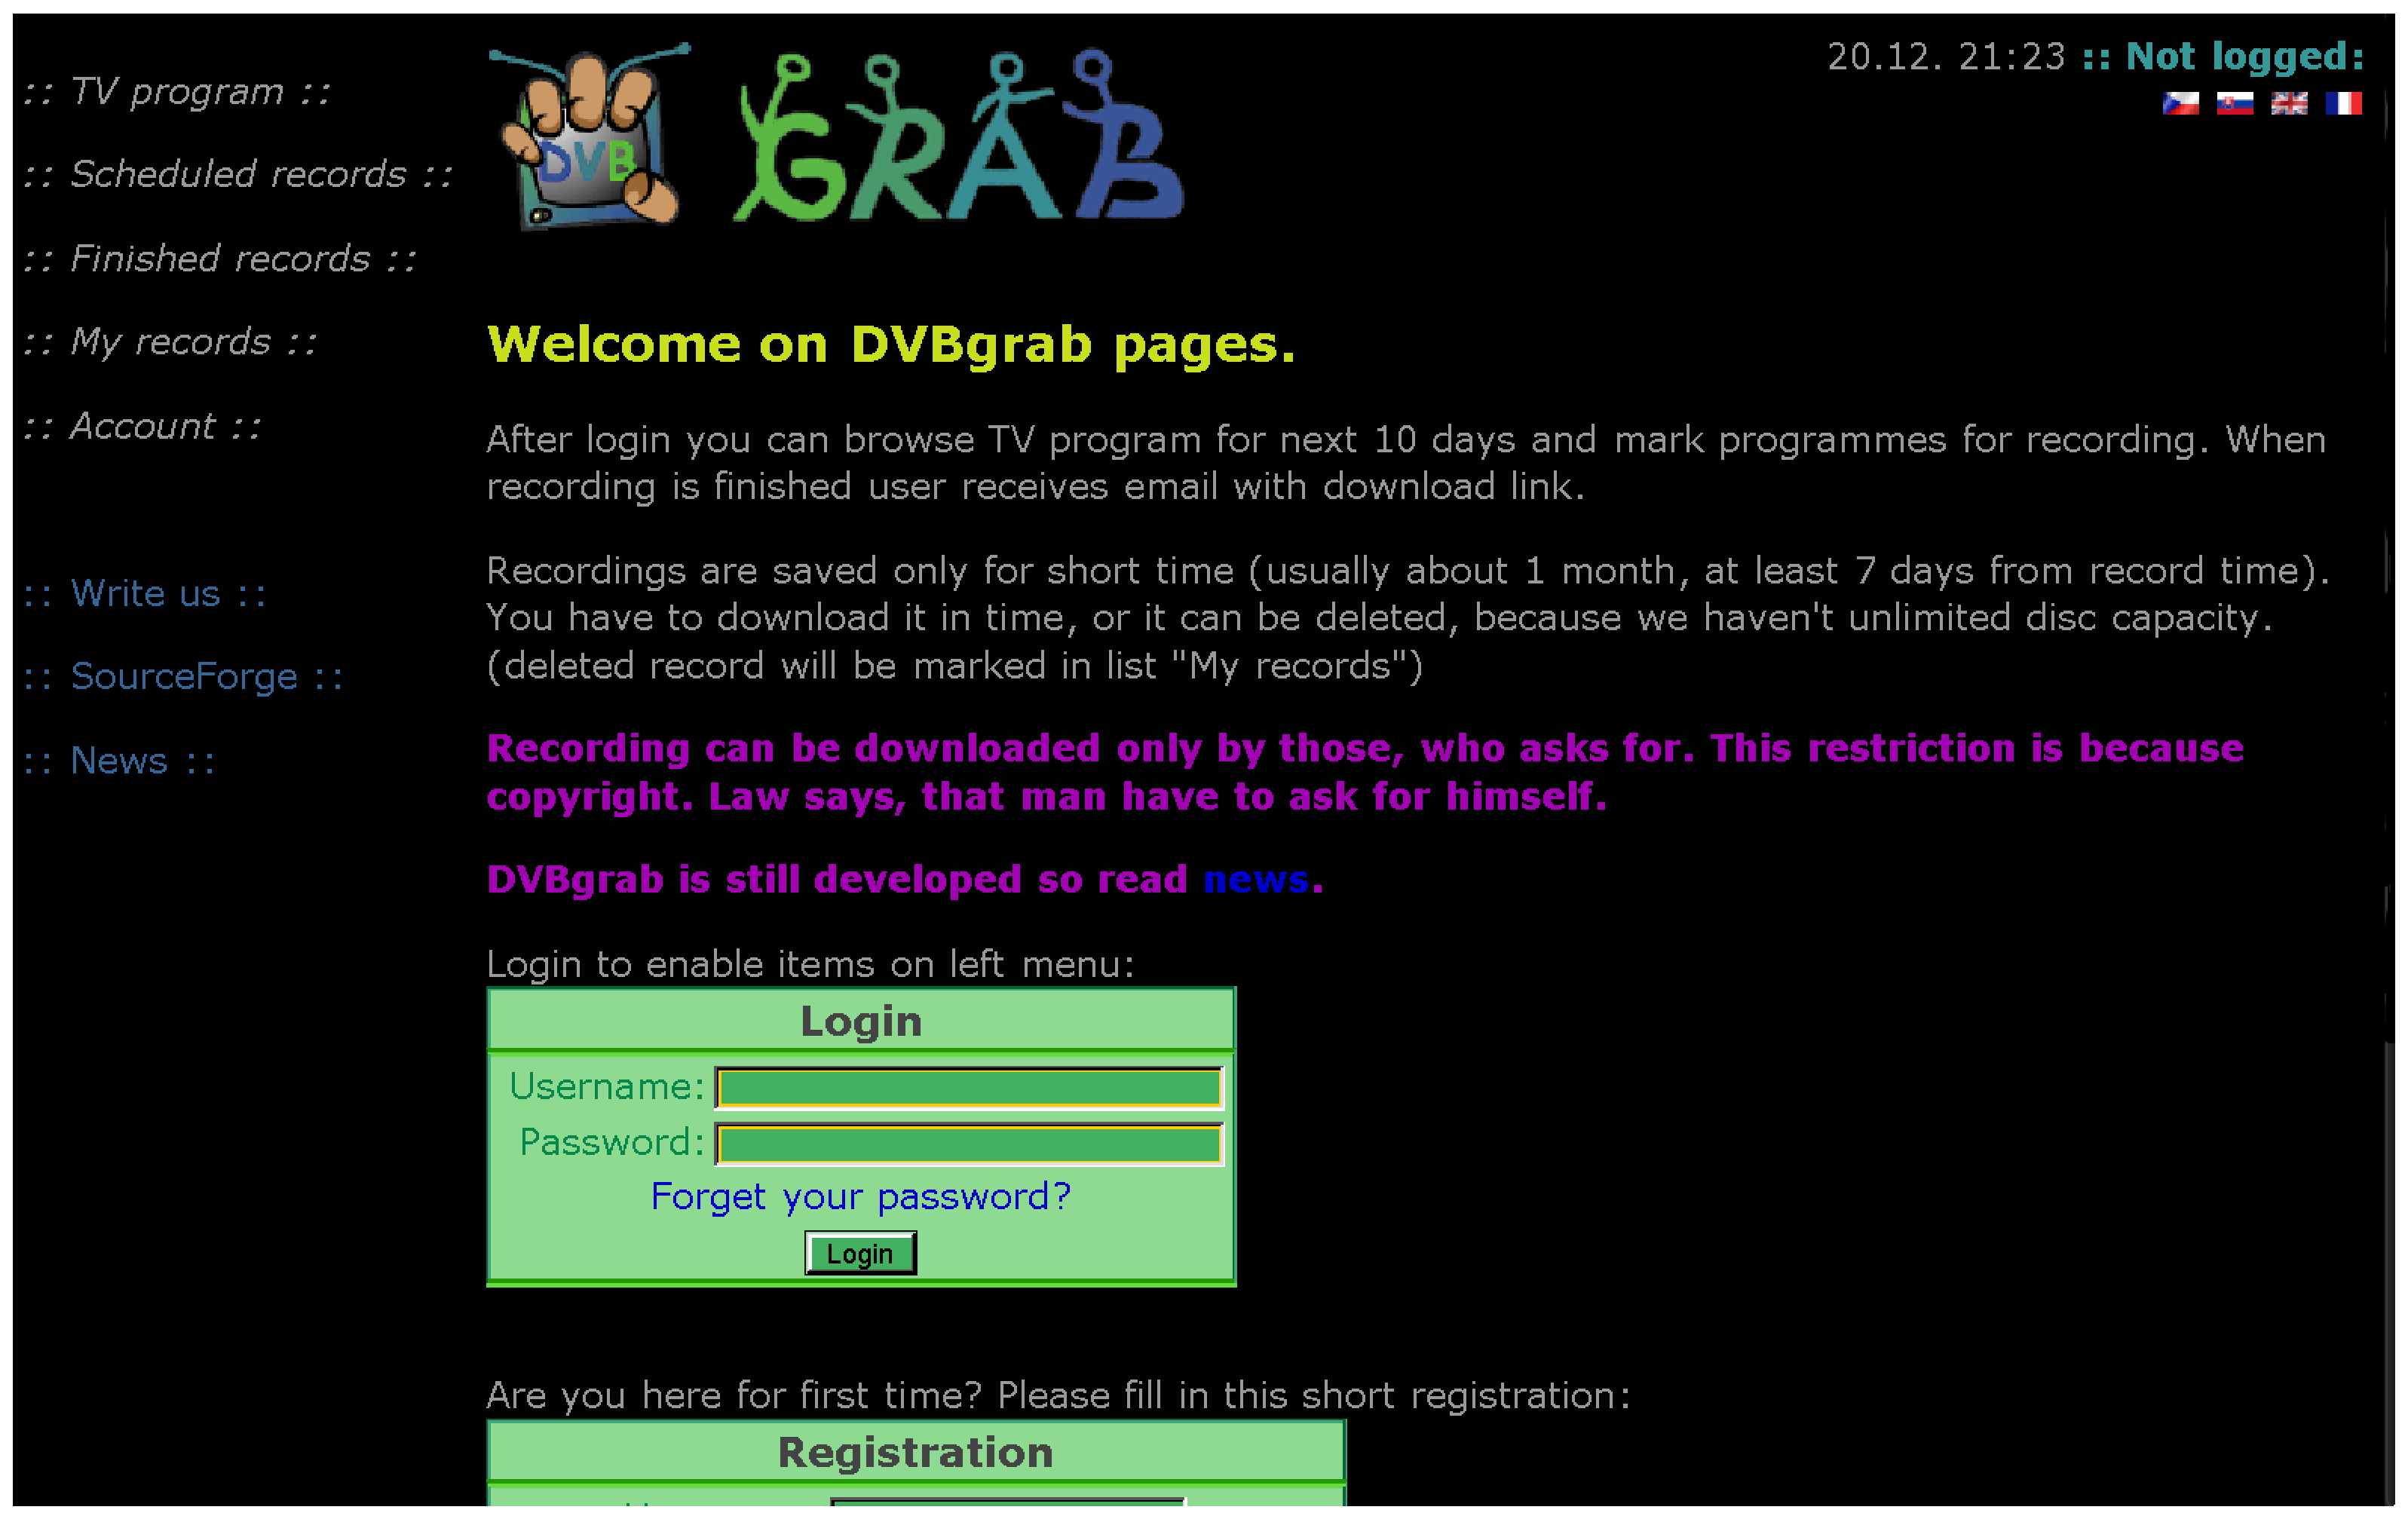
\includegraphics[width=12cm]{images/scrPrihlaseni}
\caption{Ukázka přihlášení}
\label{fig:scr1}
\end{center}
\end{figure}

\nopagebreak 

\begin{figure}[ht]
\begin{center}
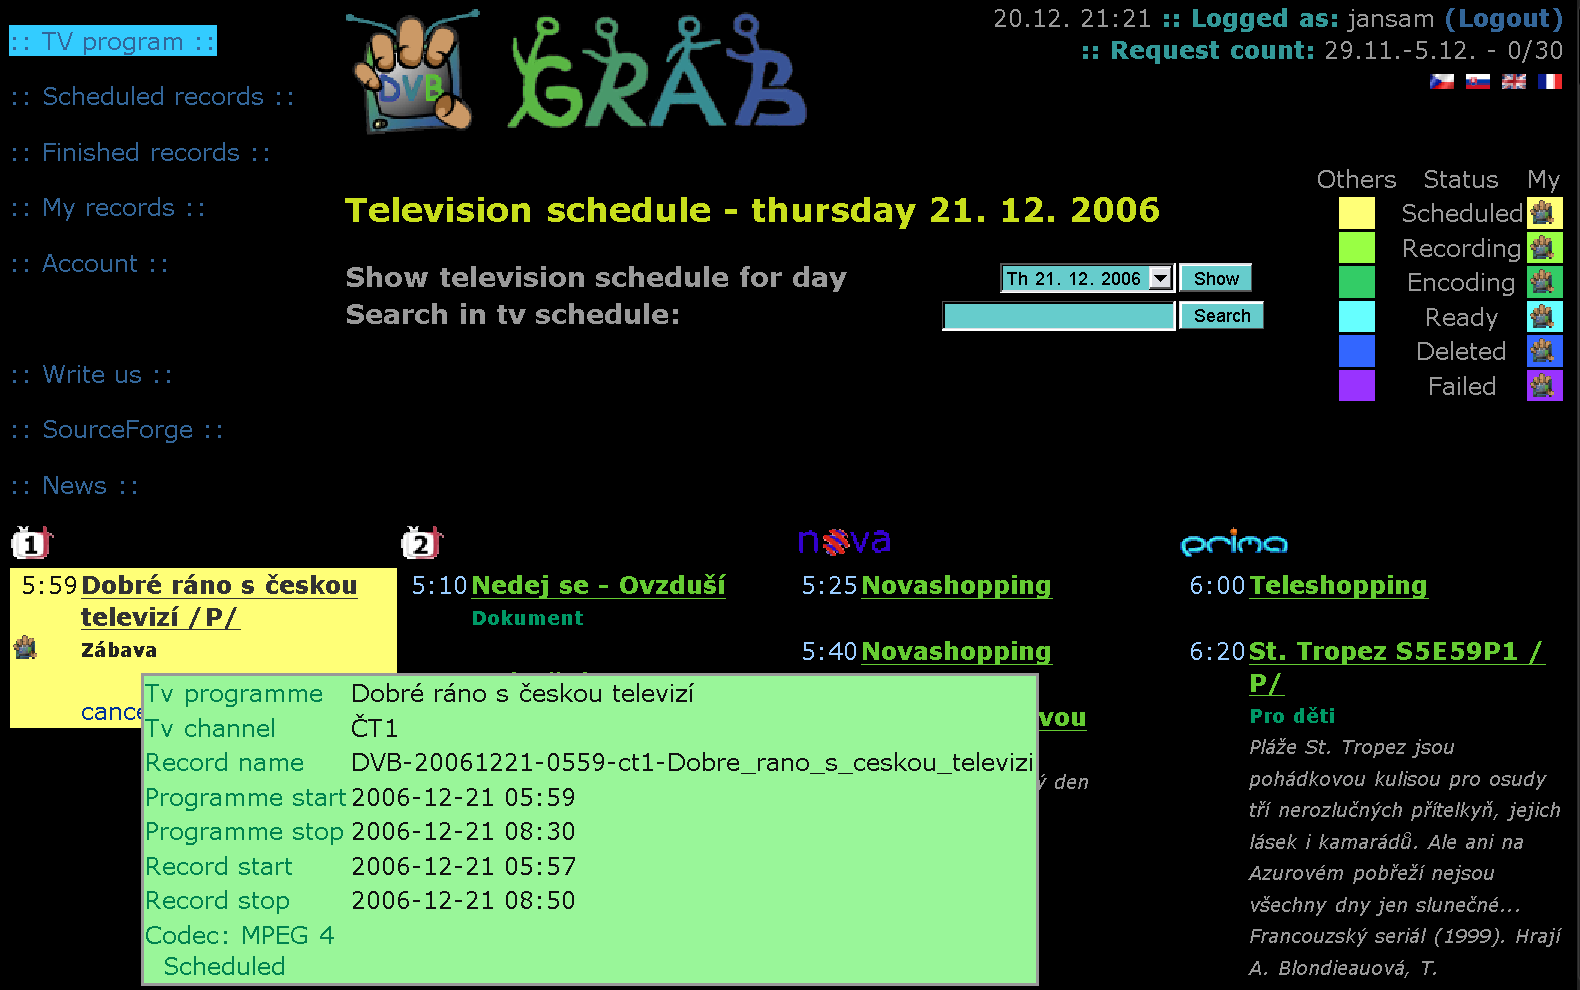
\includegraphics[width=12cm]{images/scrProgram}
\caption{Ukázka programu}
\label{fig:scr2}
\end{center}
\end{figure}

\vfil
\pagebreak

\begin{figure}[ht]
\begin{center}
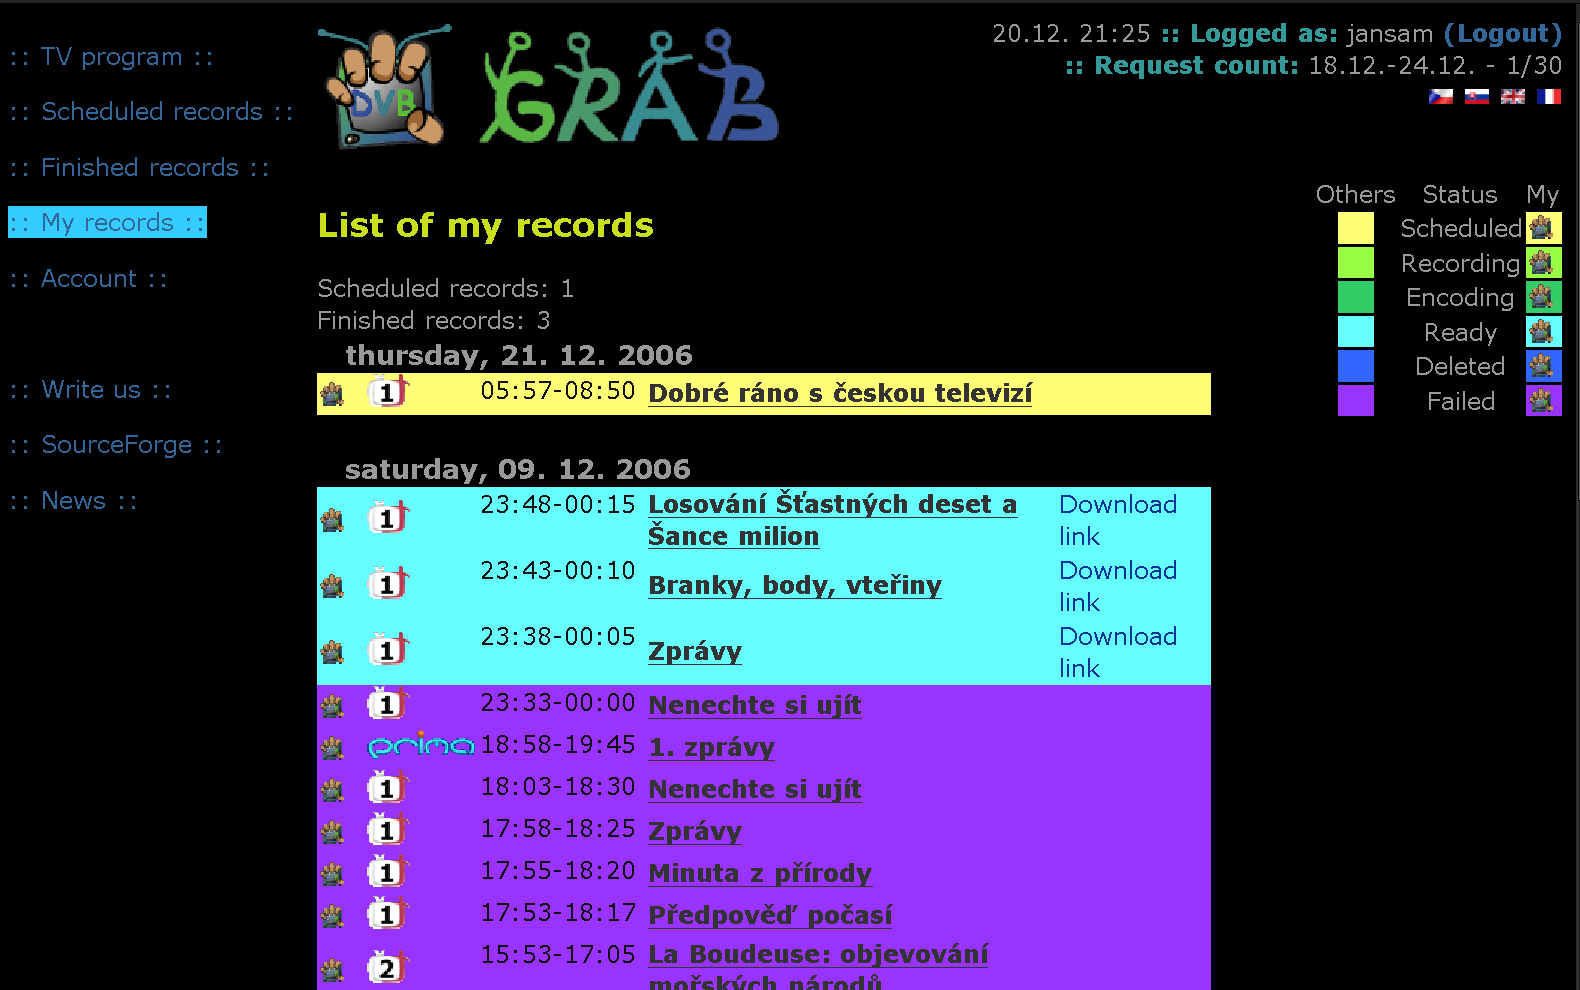
\includegraphics[width=12cm]{images/scrSeznam}
\caption{Ukázka seznamu grabů}
\label{fig:scr3}
\end{center}
\end{figure}

\begin{figure}[ht]
\begin{center}
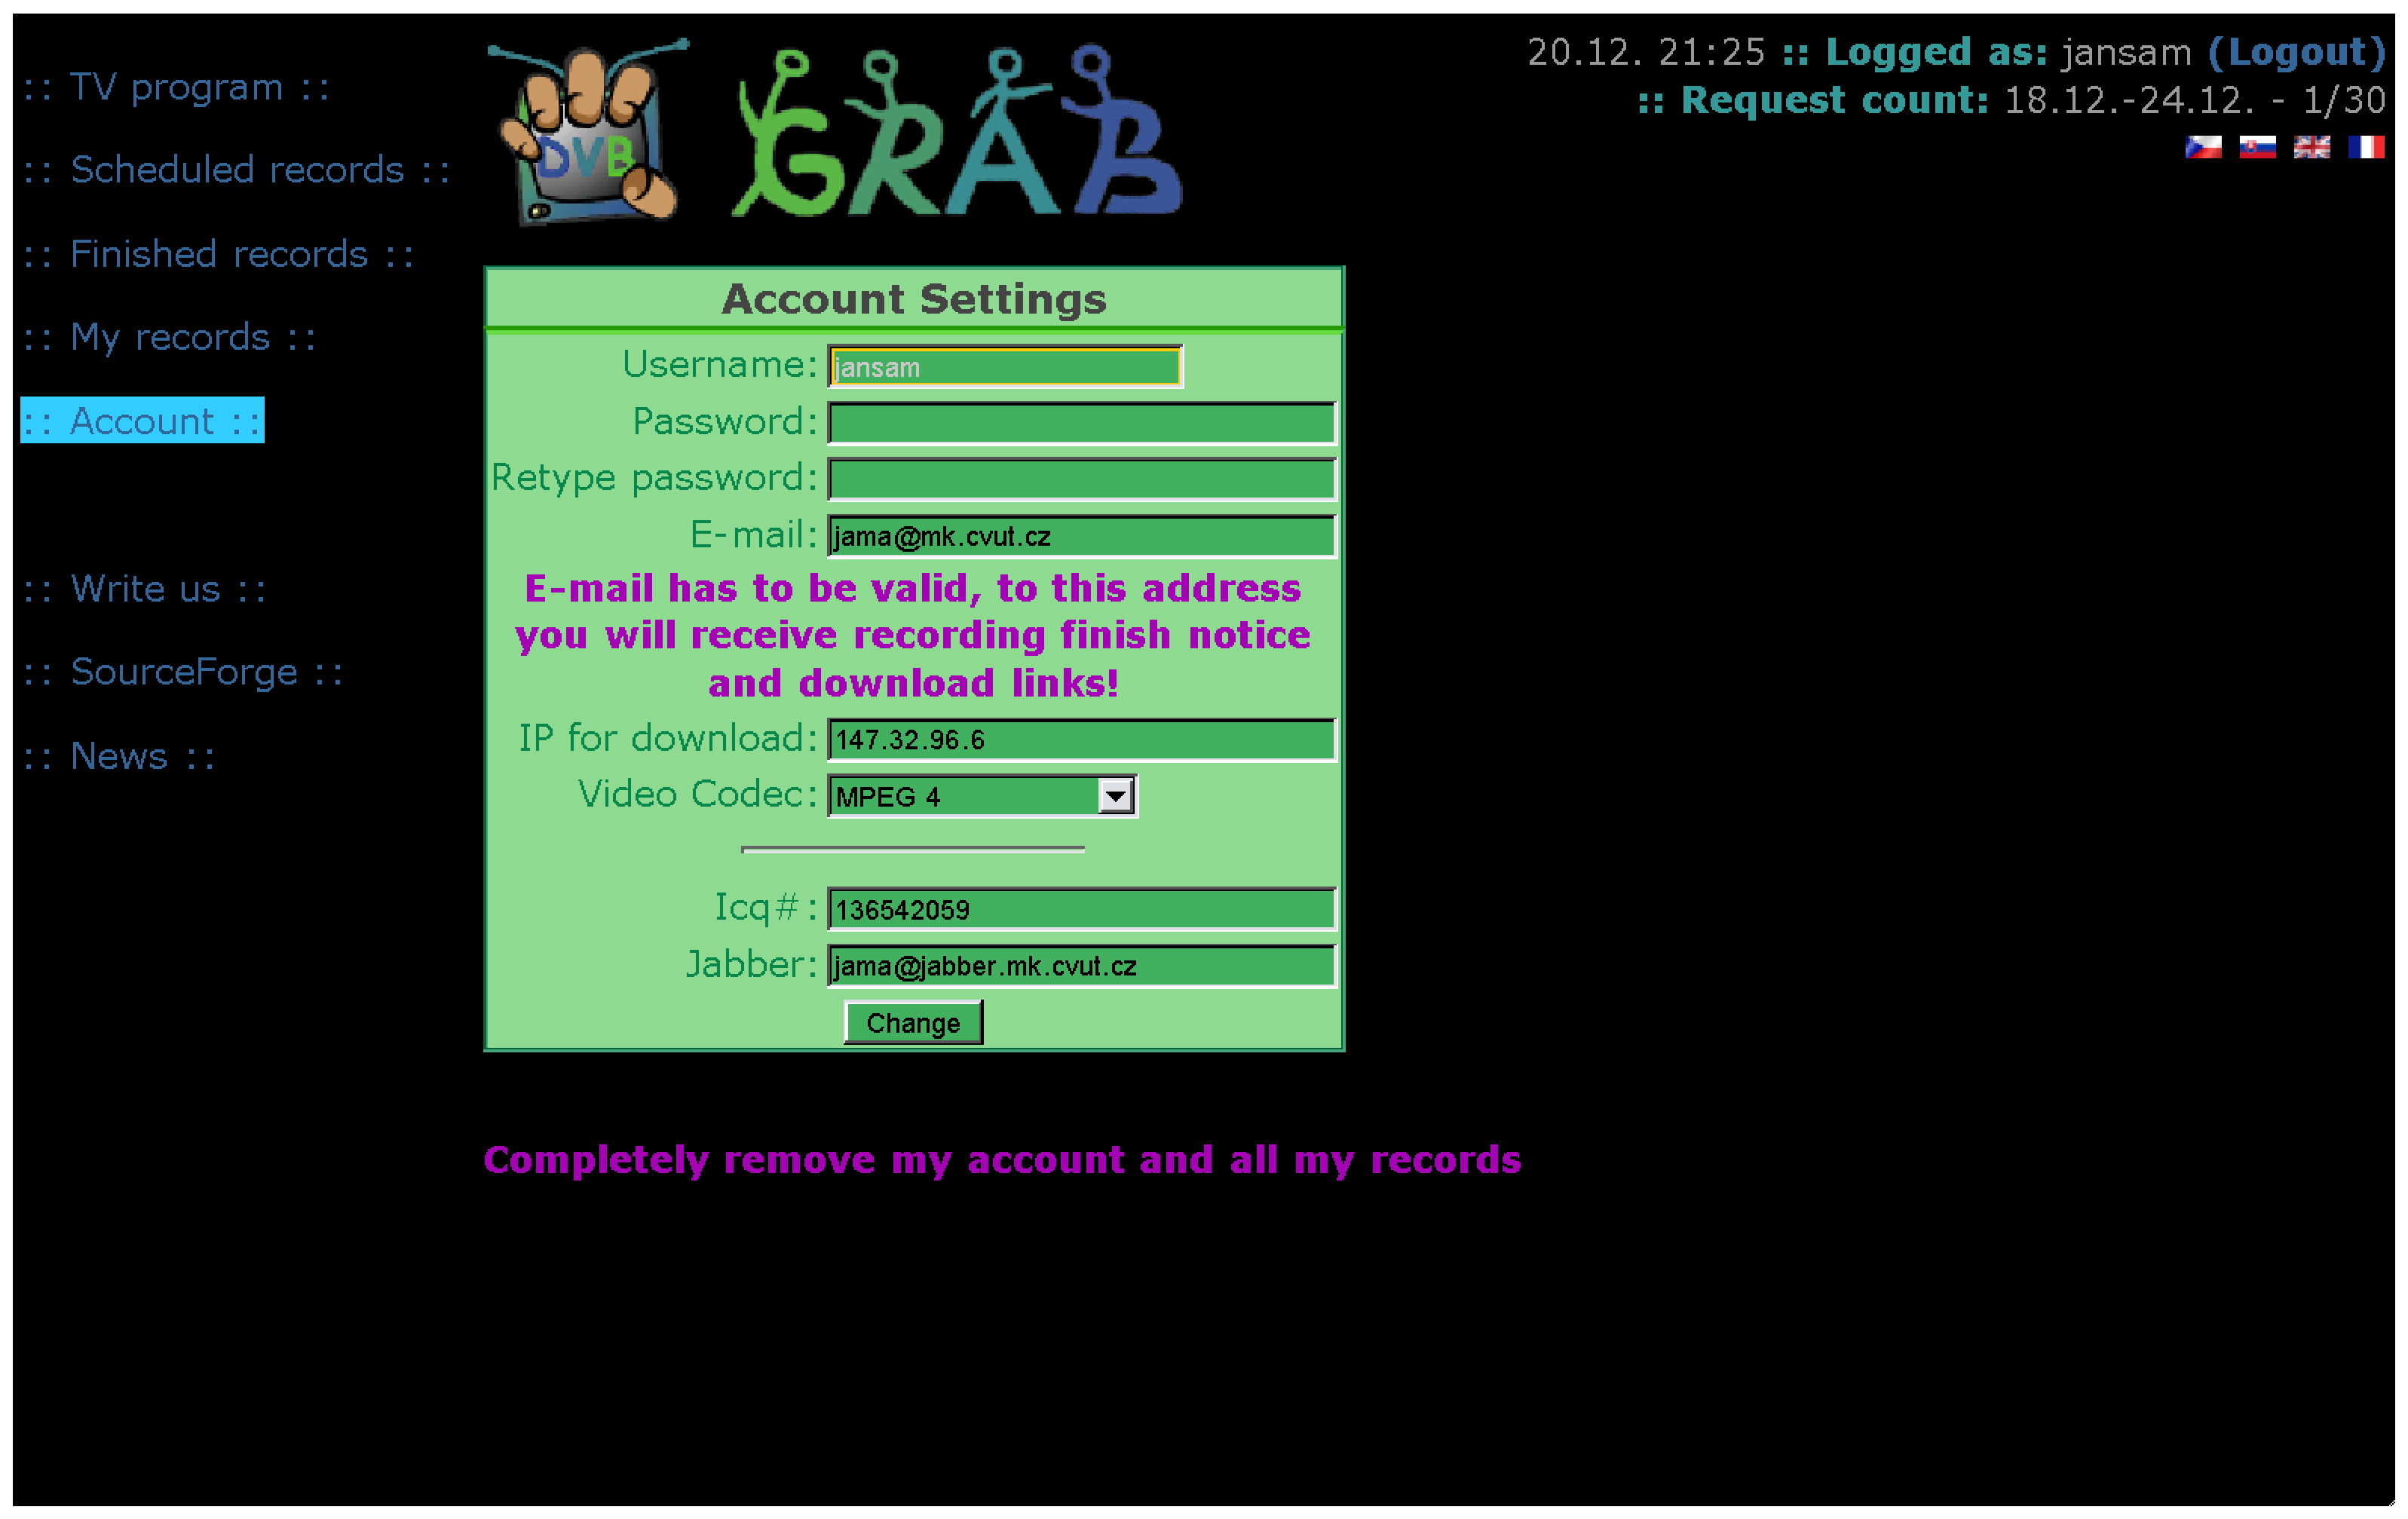
\includegraphics[width=12cm]{images/scrNastaveni}
\caption{Ukázka nastavení účtu}
\label{fig:scr4}
\end{center}
\end{figure}

\vfil
\pagebreak

\cleardoublepage
%*************************************************************************

\chapter{Formáty pro ukládání audio-video}
Audio-video data se ukládájí v souborovém a přenášejí v síťovém formátu, obecně tomu říkáme kontejner. Kontejner zajišťuje synchronizaci různých složek (audio, video, titulky) a může podporovat například různé kapitoly v rámci jednoho souboru (známé z DVD). Kontejner umí pracovat s určitými typy audio a video kodeků. Kodeky určují, jakým způsobem jsou data digitalně uložena. 
\section{Organizace ovlivňující audio-video formáty současnosti}
\bitem
\item\textbf{MPEG} -- Motion Pictures Expert Group je název standardizační skupiny ISO. V normách je v různých částech vždy obsažena definice jak kontejneru, tak audio i video kodeků.
\item\textbf{VCEG} -- Video Coding Experts Group, skupina pro návrh audio-video standardu skupiny ITU-T.
\item\textbf{Firmy Microsoft, Apple a další}
\item\textbf{Neziskové organizace a dobrovolníci vytvářející svobodné implementace, obvykle kompatibilní s některým standardem.}
\eitem
\section{Nejznámější kontejnery}
\bitem
\item\textbf{MPEG-1} -- Je nejstarším standardem, využívá se například u Video CD (VCD). Jeho kvalita je zhruba srovnatelná s kvalitou záznamu na analogové VHS kazetě. Součástí toho standardu je i známý audio kodek MP3, což je zkratka za MPEG-1 Part 3 Layer 3 (MPEG-1 Audio Layer 3). Přehrávání a nahrávání tohoto formátu je hardwarově nejméně náročné a také je to formát nejvíce kompatibilní.
\item\textbf{MPEG-2} -- Nástupce MPEG-2 nově přináší podporu pro prokládané video a 2 různé kontejnery pro vkládání audio-video dat.
\item\textbf{MPEG-2 TS} -- Transport stream neboli kontejner pro přenášení signálu po méně spolehlivém kanálu, používá se například u DVB vysílání.
\item\textbf{MPEG-2 PS} -- Program stream je naopak navržen pro použití na spolehlivém médiu jako je DVD a SuperVideo CD (SVCD).
\item\textbf{MPEG-2 VOB} -- Rozšíření MPEG-2 používané na DVD discích. Umožňuje definovat jednotlivé kapitoly, podpora pro titulky ve formátu VobSub a také pro ne-MPEG audio kodeky, jako je často používaný AC3 pro prostorový zvuk 5.1.
\item\textbf{MPEG-3} -- Původně definovaný pro televizní vysílání s vysokým rozlišením HDTV. Místo tohoto formátu se pro HDTV používá mírně vylepšený MPEG-2.
\item\textbf{MPEG-4 MP4} -- Nejnovější formát z rodiny MPEG standardů. Největším rozdílem proti předchůdcům je použití kodeků s vysokou kompresí pro audio i video. Také je zahrnuta podpora pro systém ochrany autorských práv DRM (Digital Rights Management). Používá se nejčasteji pro uchování audio-video na počítači a tam, kde je třeba zajistit co nejmenší datový tok, třeba u DVB vysílání pro přenosná zařízení (DVB-H). Definuje 2 skupiny video kodeků s vysokou kompresí MPEG-4 ASP a MPEG-4 AVC.
\item\textbf{AVI} -- Audio Video Interleave, souborový kontejner navržený firmou Microsoft podobný formátu MPEG-4.
\item\textbf{ASF} -- Advanced Systems Format, dříve Advanced Streaming Format, přenosový kontejner navržený firmou Microsoft.
\item\textbf{QuickTime} -- Kontejner od firmy Apple. Používá přípony .mov a .qt. Byl základem pro tvorbu standardu MP4.
\item\textbf{OGG/OGM} -- Svobodná varianta vyvinutá v organizaci Xiph.Org \cite{xiphURL}.
\item\textbf{Matroska} -- Další svobodná varianta s popisem složek ve formátu EBML (Extensible Binary Meta Language -- binární obdoba XML). Podobá se QuickTime, MP4 a ASF.
\item\textbf{3GP} -- Převážně pro přenosná zařízení jako telefony a PDA navržený organizací 3GPP.
\item\textbf{NUT} -- Z projektu MPlayer/FFmpeg.
\item\textbf{FLV} -- Video z Flash playeru od Adobe.
\item\textbf{RealMedia}
\item\textbf{...}
\eitem
\section{Nejpoužívanější video kodeky}
\bitem
\item\textbf{MPEG-1 Video} -- Nejstarší a vhodný spíše pro video s nízkým rozlišením, podporuje pouze neprokládané video (progressive scan).
\item\textbf{MPEG-2 Video} -- Kompatibilní s MPEG-1 Video, ale při toku více než 3Mbit/s již efektivnější a také podporuje prokládané video (interlaced) známé z televizního vysílání. Definuje různé profily (typy snímků P, I, B; rozložení YUV a kanálů) a úrovně (rozlišení, framerate, bitrate). Kombinací profilů a levelů získáme škálu různě kvalitních variant použitelných od bezdrátových zařízení po kvalitní zařízení pro vysoké rozlišení (HD).
\item\textbf{MPEG-4 ASP} -- Advanced Simple Profile, odpovídá standardu VCEG H.263 (implementace XviD, DivX, 3ivx, QuickTime, libavcodec).
\item\textbf{MPEG-4 AVC} -- Advanced Video Coding, vznikl spoluprácí skupin MPEG a VCEG a~odpovídá H.264 (implementace x264, libavcodec). Používán pro DVD s vysokým rozlišením (HD DVD) a pravděpodobně použitý pro Blu-ray video disky. Lze také použít pro vysílání DVB ve vysokém rozlišení.
\item\textbf{Theora} -- Svobodný kodek kvalitativně srovnatelný s MPEG-4 ASP i MPEG-4 AVC.
\item\textbf{WMV} -- Windows Media Video, odpověd Microsoftu na kodeky MPEG-4 ASP.
\item\textbf{RealVideo}
\item\textbf{MJPEG}
\item\textbf{...}
\eitem
\section{Nejpoužívanější audio kodeky}
\bitem
\item\textbf{MPEG-1 Layer 2 Audio} -- Nižší komprese.
\item\textbf{MPEG-1 Layer 3 Audio} -- Vyšší ztrátová komprese, rozšířená podpora v přehrávačích, známý jako MP3.
\item\textbf{AAC} -- Advanced Audio Coding, definovaný v MPEG-2 část 7 a MPEG-4 část 3 (podle implementace).
\item\textbf{AC3} -- Adaptive Transform Coder 3, až 6 kanálový zvuk Dolby Digital.
\item\textbf{FLAC} -- Free Lossless Audio Codec, svobodná alternativa bezeztrátového audio kodeku.
\item\textbf{Vorbis} -- Svobodná náhrada kodeku MP3, také se ztrátovou kompresí.
\item\textbf{Speex} -- Svobodný se ztrátovou kompresí optimalizován pro uchování a přenos lidské řeči.
\item\textbf{WMA}
\item\textbf{RealAudio}
\item\textbf{ATRAC}
\item\textbf{...}
\eitem


\cleardoublepage
%*************************************************************************


\chapter{Slovník pojmů}
\begin{description}
\item[DVB] Digital Video Broadcasting
\item[MPEG] Motion Pictures Expert Group
\item[Xiph] Xiph.Org sdružení pro podporu vývoje svobodných formátů a protokolů
\item[GRAB] Záznam z TV, nebo jineho zdroje
\item[QAM] Quadrature Amplitude Modulation
\item[OFDM] Orthogonal Frequency Division Multiplexing
\item[QPSK] Quaternary Phase-Shift Keying 
\item[FEC] Forward Error Correction 
\item[VLS] VideoLAN Server 
\item[VLC] VideoLAN Client 
\item[VLM] VideoLAN Client v režimu VideoLAN Manager 
\end{description}


\cleardoublepage
%*************************************************************************

\twocolumn
\chapter{Obsah přiloženého CD}
\textbf{dp:}
\bitem
\item dp\_bibliography.bib
\item dp\_cd.tex
\item dp\_format.cls
\item dp\_formaty.tex
\item dp\_instalace.tex
\item dp\_macro.tex
\item dp\_ocekavame.tex
\item dp.pdf
\item dp\_pojmy.tex
\item dp\_popis.tex
\item dp\_pouziti.tex
\item dp\_prijem.tex
\item dp\_testovani.tex
\item dp.tex
\item dp\_udrzba.tex
\item dp\_vysilani.tex
\item dp\_zaver.tex
\item images
\item Makefile
\eitem
\textbf{dp/images:}
\bitem
\item dvbgrab.dia
\item dvbgrab.eps
\item dvbgrab.png
\item LogoK336.eps
\item PATaPMT.eps
\item scrNastaveni.eps
\item scrNastaveni.png
\item scrPrihlaseni.eps
\item scrPrihlaseni.png
\item scrProgram.eps
\item scrProgram.png
\item scrSeznam.eps
\item scrSeznam.png
\item videolan.eps
\eitem
\textbf{dvbgrab:}
\bitem
\item account.inc.php
\item account.php
\item actions.php
\item adodb
\item authenticate.php
\item authentication.php
\item backend
\item config.php
\item config.php.dist
\item configure.sh
\item const.php
\item css
\item docs
\item dolib.inc.php
\item dvbgrab\_service
\item footer.php
\item grabinfoJS.php
\item grabinfo.php
\item header.inc.php
\item header.php
\item charset.inc.php
\item images
\item index.php
\item lang
\item language.accept.inc.php
\item language.inc.php
\item legend.inc.php
\item listtv.php
\item log
\item loggers.inc.php
\item menu.php
\item news.php
\item plan.php
\item project-web
\item screenshot1.png
\item screenshot1.xcf
\item screenshot2.png
\item screenshot3.png
\item screenshot4.png
\item search.php
\item secure.sh
\item sendPass.php
\item service
\item setup.php
\item sql
\item status.inc.php
\item telinfoJS.php
\item telinfo.php
\item tvgrabbers
\item tvprog.php
\item users
\item view.inc.php
\vfil
\eitem
\textbf{dvbgrab/backend:}
\bitem
\item adodb
\item clean.inc.php
\item clean.php
\item config.php
\item dolib.inc.php
\item encode\_loop.php
\item encode\_process.php
\item encode\_queue\_print.php
\item encode\_queue\_restore.php
\item encoders
\item grab\_loop.php
\item grab\_process.php
\item charset.inc.php
\item lang
\item loggers.inc.php
\item output.inc.php
\item print\_xsl\_template.php
\item send\_daily\_report.php
\item send\_user\_info.php
\item status.inc.php
\eitem
\textbf{dvbgrab/backend/encoders:}
\bitem
\item mpeg2.sh
\item mpeg4-full.sh
\item mpeg4-medium.sh
\item mpeg4.sh
\item mpeg4-small.sh
\eitem
\textbf{dvbgrab/css:}
\bitem
\item dvbgrab.css
\eitem
\textbf{dvbgrab/docs:}
\bitem
\item AUTHORS
\item COPYING
\item COPYRIGHT
\item CHANGES
\item INSTALL
\item README
\item TODO
\eitem
\textbf{dvbgrab/images:}
\bitem
\item cs.gif
\item dot.gif
\item dot.xcf
\item en.gif
\item fr.gif
\item grab.gif
\item grab2.gif
\item loading.gif
\item logos
\item minus.gif
\item plus.gif
\item sk.gif
\item top.black.png
\item top.full.png
\item top.gif
\item top.half.png
\item top.png
\item top.xcf
\eitem
\textbf{dvbgrab/images/logos:}
\bitem
\item ct1p.gif
\item ct1.png
\item ct2p.gif
\item ct2.png
\item novap.gif
\item nova.png
\item ockop.gif
\item primap.gif
\item prima.png
\eitem
\textbf{dvbgrab/lang:}
\bitem
\item lang.cs.inc.php
\item lang.en.inc.php
\item lang.fr.inc.php
\item lang.sk.inc.php
\eitem
\textbf{dvbgrab/log:}

\textbf{dvbgrab/project-web:}
\bitem
\item css
\item footer.php
\item header.inc.php
\item header.php
\item images
\item index.php
\item menu.php
\eitem
\onecolumn
\textbf{dvbgrab/project-web/css:}
\bitem
\item dvbgrab.css
\eitem
\textbf{dvbgrab/project-web/images:}
\bitem
\item top.png
\eitem
\textbf{dvbgrab/service:}
\bitem
\item dvbgrab
\item README
\item vlm
\item vlm.cfg
\item vlm.cfg.human.readable
\eitem
\textbf{dvbgrab/sql:}
\bitem
\item convert.sh
\item data.sql
\item mysql.sql
\item postgres.sql
\eitem
\textbf{dvbgrab/tvgrabbers:}
\bitem
\item func.inc.php
\item tv\_grab\_novinky\_cz
\item xmltv\_to\_db.php
\eitem
\textbf{dvbgrab/tvgrabbers/tv\_grab\_novinky\_cz:}
\bitem
\item tv\_grab\_novinky\_cz.php
\item uget.inc.php
\eitem
\textbf{dvbgrab/users:}
\bitem
\item index.php
\eitem
\vfil

\cleardoublepage
%*************************************************************************

\end{document}
